\chapter{Preventivo}

\section{Verso la RTB}

\subsection{Primo periodo}

In questa fase i ruoli da ricoprire per portare a termine gli obiettivi
pianificati sono:
\begin{itemize}
    \item \textit{Responsabile};
    \item \textit{Amministratore};
    \item \textit{Verificatore}.
\end{itemize}

\subsubsection{Preventivo orario}

\begin{table}[H]
    \renewcommand\arraystretch{1.5}
    \centering
    \begin{tabular}{|l|c|c|c|c|c|c|c|}
    \hline
    \rowcolor[HTML]{036400}
    \textcolor{white}{\textbf{Membro}} & \multicolumn{1}{l|}{\textcolor{white}{\textbf{RE}}} & \multicolumn{1}{l|}{\textcolor{white}{\textbf{AM}}} & \multicolumn{1}{l|}{\textcolor{white}{\textbf{AN}}} & \multicolumn{1}{l|}{\textcolor{white}{\textbf{PT}}} & \multicolumn{1}{l|}{\textcolor{white}{\textbf{PR}}} & \multicolumn{1}{l|}{\textcolor{white}{\textbf{VE}}} & \multicolumn{1}{l|}{\textcolor{white}{\textbf{Totale ore persona}}} \\ \hline
    \rowcolor[HTML]{EFEFEF}\textit{Marco Mazzucato}  & 2 & 3  & - & - & - & 1 & 6  \\ \hline
    \rowcolor[HTML]{C0C0C0}\textit{Marco Mamprin}    & - & 3  & - & - & - & 1 & 4  \\ \hline
    \rowcolor[HTML]{EFEFEF}\textit{Marko Vukovic}    & 2 & 3  & - & - & - & 1 & 6  \\ \hline
    \rowcolor[HTML]{C0C0C0}\textit{Mattia Zanellato} & - & 3  & - & - & - & 1 & 4  \\ \hline
    \rowcolor[HTML]{EFEFEF}\textit{Emanuele Pase}    & - & 3  & - & - & - & 1 & 4  \\ \hline
    \rowcolor[HTML]{C0C0C0}\textit{Riccardo Contin}  & - & 3  & - & - & - & 1 & 4  \\ \hline
    \rowcolor[HTML]{EFEFEF}\textit{Lorenzo Onelia}   & - & 3  & - & - & - & 1 & 4  \\ \hline
    \textbf{Totale ore ruolo} & 4 & 21 & - & - & - & 7 & 32 \\ \hline
    \end{tabular}
    \caption{Distribuzione delle ore per la prima milestone}
\end{table}

\begin{figure}[H]
    \includegraphics[width=1.0\textwidth]{Istogramma1.jpg}
    \caption{Istogramma della distribuzione delle ore per la prima milestone}
\end{figure}

\begin{figure}[H]
    \includegraphics[width=1.0\textwidth]{Torta1.1.jpg}
    \caption{Grafico a torta della distribuzione delle ore per la prima milestone}
\end{figure}

\newpage
\subsubsection{Preventivo economico}

\begin{table}[H]
    \renewcommand\arraystretch{1.5}
    \centering
    \begin{tabular}{|l|c|c|}
    \hline
    \rowcolor[HTML]{036400}
    \textcolor{white}{\textbf{Ruolo}} & \multicolumn{1}{l|}{\textcolor{white}{\textbf{Ore}}} & \multicolumn{1}{l|}{\textcolor{white}{\textbf{Costo (€)}}} \\ \hline
    \rowcolor[HTML]{EFEFEF}\textit{Responsabile} & 4 & 120 \\ \hline
    \rowcolor[HTML]{C0C0C0}\textit{Amministratore} & 21 & 420 \\ \hline
    \rowcolor[HTML]{EFEFEF}\textit{Analista} & - & - \\ \hline
    \rowcolor[HTML]{C0C0C0}\textit{Progettista} & - & - \\ \hline
    \rowcolor[HTML]{EFEFEF}\textit{Programmatore} & - & - \\ \hline
    \rowcolor[HTML]{C0C0C0}\textit{Verificatore} & 7 & 105 \\ \hline
    \rowcolor[HTML]{EFEFEF}\textbf{Totale} & 32 & 645 \\ \hline
    \end{tabular}
    \caption{Prospetto dei costi per la prima milestone}
\end{table}

\begin{figure}[H]
    \includegraphics[width=1.0\textwidth]{Torta1.2.jpg}
    \caption{Grafico a torta della distribuzione dei costi per la prima milestone}
\end{figure}

\newpage
\subsection{Secondo periodo}

In questa fase i ruoli da ricoprire per portare a termine gli obiettivi
pianificati sono:
\begin{itemize}
    \item \textit{Responsabile};
    \item \textit{Amministratore};
    \item \textit{Analista};
    \item \textit{Verificatore}.
\end{itemize}

\subsubsection{Preventivo orario}

\begin{table}[H]
    \renewcommand\arraystretch{1.5}
    \centering
    \begin{tabular}{|l|c|c|c|c|c|c|c|}
    \hline
    \rowcolor[HTML]{036400}
    \textcolor{white}{\textbf{Membro}} & \multicolumn{1}{l|}{\textcolor{white}{\textbf{RE}}} & \multicolumn{1}{l|}{\textcolor{white}{\textbf{AM}}} & \multicolumn{1}{l|}{\textcolor{white}{\textbf{AN}}} & \multicolumn{1}{l|}{\textcolor{white}{\textbf{PT}}} & \multicolumn{1}{l|}{\textcolor{white}{\textbf{PR}}} & \multicolumn{1}{l|}{\textcolor{white}{\textbf{VE}}} & \multicolumn{1}{l|}{\textcolor{white}{\textbf{Totale ore persona}}} \\ \hline
    \rowcolor[HTML]{EFEFEF}\textit{Marco Mazzucato}  & - & 2   & 2  & - & - & 2  & 6   \\ \hline
    \rowcolor[HTML]{C0C0C0}\textit{Marco Mamprin}    & - & 2   & 1  & - & - & 2  & 5   \\ \hline
    \rowcolor[HTML]{EFEFEF}\textit{Marko Vukovic}    & - & 1.5 & 3  & - & - & 3  & 7.5 \\ \hline
    \rowcolor[HTML]{C0C0C0}\textit{Mattia Zanellato} & - & -   & 3  & - & - & 3  & 6   \\ \hline
    \rowcolor[HTML]{EFEFEF}\textit{Emanuele Pase}    & - & -   & 3  & - & - & 3  & 6   \\ \hline
    \rowcolor[HTML]{C0C0C0}\textit{Riccardo Contin}  & 4 & -   & 3  & - & - & 1  & 8   \\ \hline
    \rowcolor[HTML]{EFEFEF}\textit{Lorenzo Onelia}   & - & 2   & 2  & - & - & 3  & 7   \\ \hline
    \rowcolor[HTML]{C0C0C0}\textbf{Totale ore ruolo} & 4 & 7.5 & 17 & - & - & 17 & 45.5\\ \hline
    \end{tabular}
    \caption{Distribuzione delle ore per la seconda milestone}
\end{table}

\begin{figure}[H]
    \includegraphics[width=1.0\textwidth]{Istogramma2.jpg}
    \caption{Istogramma della distribuzione delle ore per la seconda milestone}
\end{figure}

\begin{figure}[H]
    \includegraphics[width=1.0\textwidth]{Torta2.1.jpg}
    \caption{Grafico a torta della distribuzione delle ore per la seconda milestone}
\end{figure}

\newpage
\subsubsection{Preventivo economico}

\begin{table}[H]
    \renewcommand\arraystretch{1.5}
    \centering
    \begin{tabular}{|l|c|c|}
    \hline
    \rowcolor[HTML]{036400}
    \textcolor{white}{\textbf{Ruolo}} & \multicolumn{1}{l|}{\textcolor{white}{\textbf{Ore}}} & \multicolumn{1}{l|}{\textcolor{white}{\textbf{Costo (€)}}} \\ \hline
    \rowcolor[HTML]{EFEFEF}\textit{Responsabile} & 4 & 120 \\ \hline
    \rowcolor[HTML]{C0C0C0}\textit{Amministratore} & 7.5 & 150 \\ \hline
    \rowcolor[HTML]{EFEFEF}\textit{Analista} & 17 & 425 \\ \hline
    \rowcolor[HTML]{C0C0C0}\textit{Progettista} & - & - \\ \hline
    \rowcolor[HTML]{EFEFEF}\textit{Programmatore} & - & - \\ \hline
    \rowcolor[HTML]{C0C0C0}\textit{Verificatore} & 17 & 255 \\ \hline
    \rowcolor[HTML]{EFEFEF}\textbf{Totale} & 45.5 & 950 \\ \hline
    \end{tabular}
    \caption{Prospetto dei costi per la seconda milestone}
\end{table}

\begin{figure}[H]
    \includegraphics[width=1.0\textwidth]{Torta2.2.jpg}
    \caption{Grafico a torta della distribuzione dei costi per la seconda milestone}
\end{figure}



\newpage
\subsection{Terzo periodo}

In questa fase i ruoli da ricoprire per portare a termine gli obiettivi
pianificati sono:
\begin{itemize}
    \item \textit{Responsabile};
    \item \textit{Amministratore};
    \item \textit{Analista};
    \item \textit{Progettista};
    \item \textit{Verificatore}.
\end{itemize}

\subsubsection{Preventivo orario}

\begin{table}[H]
    \renewcommand\arraystretch{1.5}
    \centering
    \begin{tabular}{|l|c|c|c|c|c|c|c|}
    \hline
    \rowcolor[HTML]{036400}
    \textcolor{white}{\textbf{Membro}} & \multicolumn{1}{l|}{\textcolor{white}{\textbf{RE}}} & \multicolumn{1}{l|}{\textcolor{white}{\textbf{AM}}} & \multicolumn{1}{l|}{\textcolor{white}{\textbf{AN}}} & \multicolumn{1}{l|}{\textcolor{white}{\textbf{PT}}} & \multicolumn{1}{l|}{\textcolor{white}{\textbf{PR}}} & \multicolumn{1}{l|}{\textcolor{white}{\textbf{VE}}} & \multicolumn{1}{l|}{\textcolor{white}{\textbf{Totale ore persona}}} \\ \hline
    \rowcolor[HTML]{EFEFEF}\textit{Marco Mazzucato}  & - & 1   & 1.5 & 2 & -  & 2    & 6.5  \\ \hline
    \rowcolor[HTML]{C0C0C0}\textit{Marco Mamprin}    & - & 1   & 2   & 2 & -  & 2    & 7    \\ \hline
    \rowcolor[HTML]{EFEFEF}\textit{Marko Vukovic}    & - & 1.5 & 2   & 2 & -  & 2    & 7.5  \\ \hline
    \rowcolor[HTML]{C0C0C0}\textit{Mattia Zanellato} & - & 1   & 2   & 2 & -  & 2    & 7    \\ \hline
    \rowcolor[HTML]{EFEFEF}\textit{Emanuele Pase}    & 4 & 1   & 0.5 & 2 & -  & 1    & 8.5  \\ \hline
    \rowcolor[HTML]{C0C0C0}\textit{Riccardo Contin}  & - & 1   & 1.5 & 2 & -  & 2.5  & 7    \\ \hline
    \rowcolor[HTML]{EFEFEF}\textit{Lorenzo Onelia}   & - & 1   & 1.5 & 2 & -  & 2    & 6.5  \\ \hline
    \rowcolor[HTML]{C0C0C0}\textbf{Totale ore ruolo} & 4 & 7.5 & 11  & 14& - & 13.5 & 50   \\ \hline
    \end{tabular}
    \caption{Distribuzione delle ore per la terza milestone}
\end{table}

\begin{figure}[H]
    \includegraphics[width=1.0\textwidth]{Istogramma3.jpg}
    \caption{Istogramma della distribuzione delle ore per la terza milestone}
\end{figure}

\begin{figure}[H]
    \includegraphics[width=1.0\textwidth]{Torta3.1.jpg}
    \caption{Grafico a torta della distribuzione delle ore per la terza milestone}
\end{figure}

\newpage
\subsubsection{Preventivo economico}

\begin{table}[H]
    \renewcommand\arraystretch{1.5}
    \centering
    \begin{tabular}{|l|c|c|}
    \hline
    \rowcolor[HTML]{036400}
    \textcolor{white}{\textbf{Ruolo}} & \multicolumn{1}{l|}{\textcolor{white}{\textbf{Ore}}} & \multicolumn{1}{l|}{\textcolor{white}{\textbf{Costo (€)}}} \\ \hline
    \rowcolor[HTML]{EFEFEF}\textit{Responsabile}   & 4    & 120   \\ \hline
    \rowcolor[HTML]{C0C0C0}\textit{Amministratore} & 7.5  & 150   \\ \hline
    \rowcolor[HTML]{EFEFEF}\textit{Analista}       & 11   & 275   \\ \hline
    \rowcolor[HTML]{C0C0C0}\textit{Progettista}    & 14   & 350   \\ \hline
    \rowcolor[HTML]{EFEFEF}\textit{Programmatore}  & -    & -     \\ \hline
    \rowcolor[HTML]{C0C0C0}\textit{Verificatore}   & 13.5 & 202.5 \\ \hline
    \rowcolor[HTML]{EFEFEF}\textbf{Totale}         & 50   & 1097,5\\ \hline
    \end{tabular}
    \caption{Prospetto dei costi per la terza milestone}
\end{table}

\begin{figure}[H]
    \includegraphics[width=1.0\textwidth]{Torta3.2.jpg}
    \caption{Grafico a torta della distribuzione dei costi per la terza milestone}
\end{figure}



\newpage
\subsection{Quarto periodo}

In questa fase i ruoli da ricoprire per portare a termine gli obiettivi pianificati sono:
\begin{itemize}
    \item \textit{Responsabile};
    \item \textit{Amministratore};
    \item \textit{Analista};
    \item \textit{Progettista};
    \item \textit{Programmatore};
    \item \textit{Verificatore}.
\end{itemize}

\subsubsection{Preventivo orario}

\begin{table}[H]
    \renewcommand\arraystretch{1.5}
    \centering
    \begin{tabular}{|l|c|c|c|c|c|c|c|}
    \hline
    \rowcolor[HTML]{036400}
    \textcolor{white}{\textbf{Membro}} & \multicolumn{1}{l|}{\textcolor{white}{\textbf{RE}}} & \multicolumn{1}{l|}{\textcolor{white}{\textbf{AM}}} & \multicolumn{1}{l|}{\textcolor{white}{\textbf{AN}}} & \multicolumn{1}{l|}{\textcolor{white}{\textbf{PT}}} & \multicolumn{1}{l|}{\textcolor{white}{\textbf{PR}}} & \multicolumn{1}{l|}{\textcolor{white}{\textbf{VE}}} & \multicolumn{1}{l|}{\textcolor{white}{\textbf{Totale ore persona}}} \\ \hline
    \rowcolor[HTML]{EFEFEF}\textit{Marco Mazzucato}  & - & -   & 2     & 4  & 4   & 2    & 12     \\ \hline
    \rowcolor[HTML]{C0C0C0}\textit{Marco Mamprin}    & - & 1   & 2     & 4  & 5   & 3    & 15     \\ \hline
    \rowcolor[HTML]{EFEFEF}\textit{Marko Vukovic}    & - & -   & 1     & 4  & 4   & 4    & 13     \\ \hline
    \rowcolor[HTML]{C0C0C0}\textit{Mattia Zanellato} & 4 & 4   & 1.5   & 4  & -   & 4    & 17.5   \\ \hline
    \rowcolor[HTML]{EFEFEF}\textit{Emanuele Pase}    & - & -   & -     & 3  & 4   & 3    & 10     \\ \hline
    \rowcolor[HTML]{C0C0C0}\textit{Riccardo Contin}  & - & 3   & 1     & 3  & -   & 3.5  & 10.5   \\ \hline
    \rowcolor[HTML]{EFEFEF}\textit{Lorenzo Onelia}   & - & 3   & 3     & 3  & -   & 3    & 12     \\ \hline
    \rowcolor[HTML]{C0C0C0}\textbf{Totale ore ruolo} & 4 & 11  & 10.5  & 25 & 17  & 22.5 & 90     \\ \hline
    \end{tabular}
    \caption{Distribuzione delle ore per la quarta milestone}
\end{table}

\begin{figure}[H]
    \includegraphics[width=1.0\textwidth]{Istogramma4.jpg}
    \caption{Istogramma della distribuzione delle ore per la quarta milestone}
\end{figure}

\begin{figure}[H]
    \includegraphics[width=1.0\textwidth]{Torta4.1.jpg}
    \caption{Grafico a torta della distribuzione delle ore per la quarta milestone}
\end{figure}

\newpage
\subsubsection{Preventivo economico}

\begin{table}[H]
    \renewcommand\arraystretch{1.5}
    \centering
    \begin{tabular}{|l|c|c|}
    \hline
    \rowcolor[HTML]{036400}
    \textcolor{white}{\textbf{Ruolo}} & \multicolumn{1}{l|}{\textcolor{white}{\textbf{Ore}}} & \multicolumn{1}{l|}{\textcolor{white}{\textbf{Costo (€)}}} \\ \hline
    \rowcolor[HTML]{EFEFEF}\textit{Responsabile}   & 4    & 120     \\ \hline
    \rowcolor[HTML]{C0C0C0}\textit{Amministratore} & 11   & 220     \\ \hline
    \rowcolor[HTML]{EFEFEF}\textit{Analista}       & 10.5 & 262.5   \\ \hline
    \rowcolor[HTML]{C0C0C0}\textit{Progettista}    & 25   & 625     \\ \hline
    \rowcolor[HTML]{EFEFEF}\textit{Programmatore}  & 17   & 255     \\ \hline
    \rowcolor[HTML]{C0C0C0}\textit{Verificatore}   & 22.5 & 337.5   \\ \hline
    \rowcolor[HTML]{EFEFEF}\textbf{Totale}         & 90   & 1820    \\ \hline
    \end{tabular}
    \caption{Prospetto dei costi per la quarta milestone}
\end{table}

\begin{figure}[H]
    \includegraphics[width=1.0\textwidth]{Torta4.2.jpg}
    \caption{Grafico a torta della distribuzione dei costi per la quarta milestone}
\end{figure}

\newpage
\section{Verso la PB}

\subsection{Quinto periodo}

In questa fase i ruoli da ricoprire per portare a termine gli obiettivi pianificati sono:
\begin{itemize}
    \item \textit{Responsabile};
    \item \textit{Amministratore};
    \item \textit{Analista};
    \item \textit{Progettista};
    \item \textit{Programmatore};
    \item \textit{Verificatore}.
\end{itemize}

\subsubsection{Preventivo orario}

\begin{table}[H]
    \renewcommand\arraystretch{1.5}
    \centering
    \begin{tabular}{|l|c|c|c|c|c|c|c|}
    \hline
    \rowcolor[HTML]{036400}
    \textcolor{white}{\textbf{Membro}} & \multicolumn{1}{l|}{\textcolor{white}{\textbf{RE}}} & \multicolumn{1}{l|}{\textcolor{white}{\textbf{AM}}} & \multicolumn{1}{l|}{\textcolor{white}{\textbf{AN}}} & \multicolumn{1}{l|}{\textcolor{white}{\textbf{PT}}} & \multicolumn{1}{l|}{\textcolor{white}{\textbf{PR}}} & \multicolumn{1}{l|}{\textcolor{white}{\textbf{VE}}} & \multicolumn{1}{l|}{\textcolor{white}{\textbf{Totale ore persona}}} \\ \hline
    \rowcolor[HTML]{EFEFEF}\textit{Marco Mazzucato}  & - & 1   & -     & 2    & -    & 1    & 4     \\ \hline
    \rowcolor[HTML]{C0C0C0}\textit{Marco Mamprin}    & 2 & 1   & 1     & -    & 3    & 2    & 9     \\ \hline
    \rowcolor[HTML]{EFEFEF}\textit{Marko Vukovic}    & - & 2   & -     & -    & -    & 3    & 5     \\ \hline
    \rowcolor[HTML]{C0C0C0}\textit{Mattia Zanellato} & - & -   & -     & 3.5  & 4.5  & 1    & 9     \\ \hline
    \rowcolor[HTML]{EFEFEF}\textit{Emanuele Pase}    & - & -   & -     & 2    & -    & 2    & 4     \\ \hline
    \rowcolor[HTML]{C0C0C0}\textit{Riccardo Contin}  & - & -   & -     & 2    & 2    & 2    & 6     \\ \hline
    \rowcolor[HTML]{EFEFEF}\textit{Lorenzo Onelia}   & - & 0.5 & -     & 4    & 3    & 3.5  & 11    \\ \hline
    \rowcolor[HTML]{C0C0C0}\textbf{Totale ore ruolo} & 2 & 4.5 & 1     & 13.5 & 12.5 & 14.5 & 48    \\ \hline
    \end{tabular}
    \caption{Distribuzione delle ore per la quinta milestone}
\end{table}

\begin{figure}[H]
    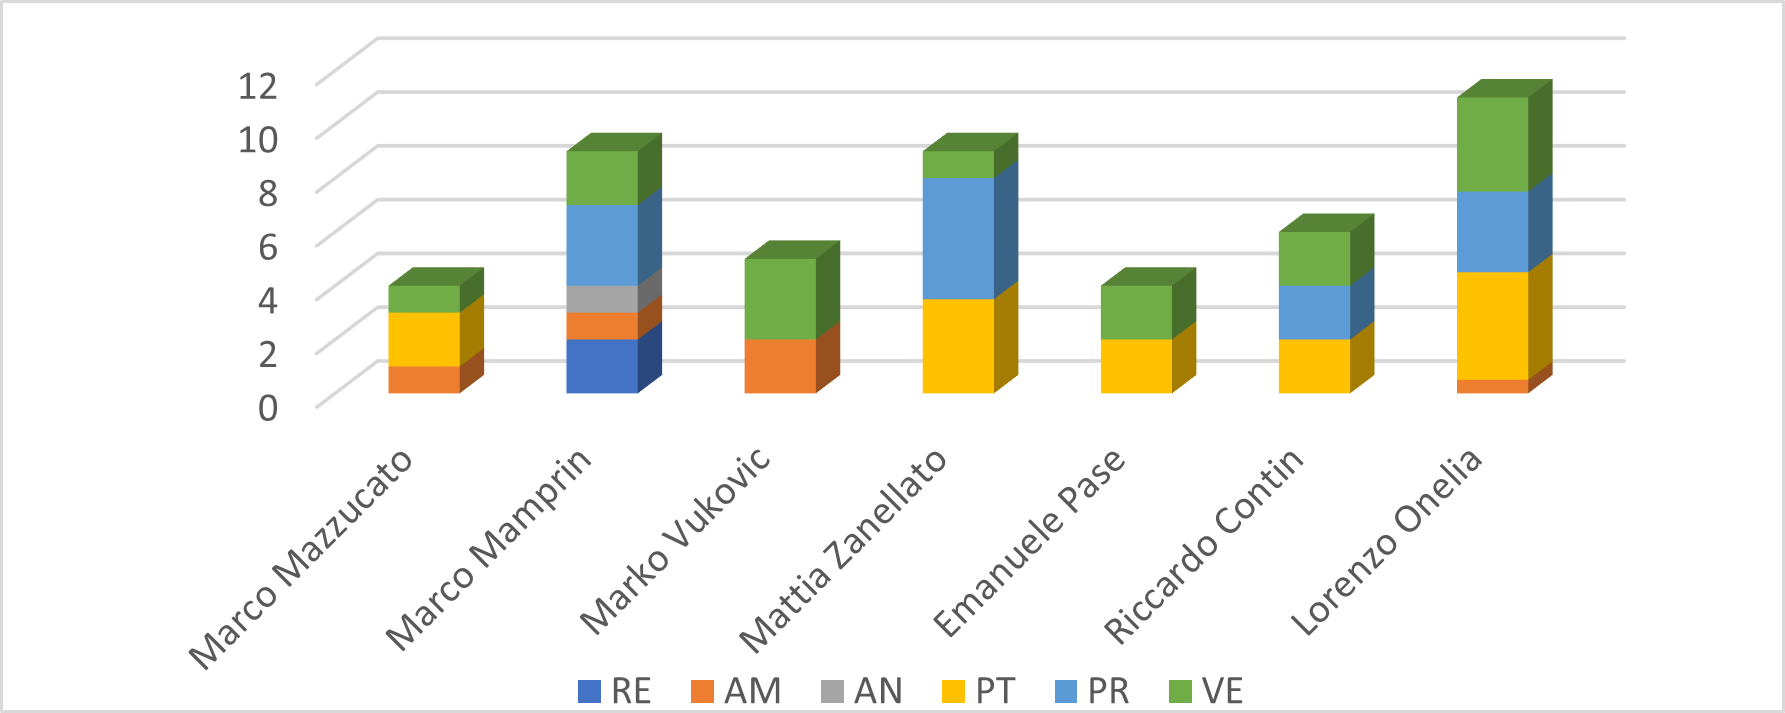
\includegraphics[width=1.0\textwidth]{Istogramma5.jpg}
    \caption{Istogramma della distribuzione delle ore per la quinta milestone}
\end{figure}

\begin{figure}[H]
    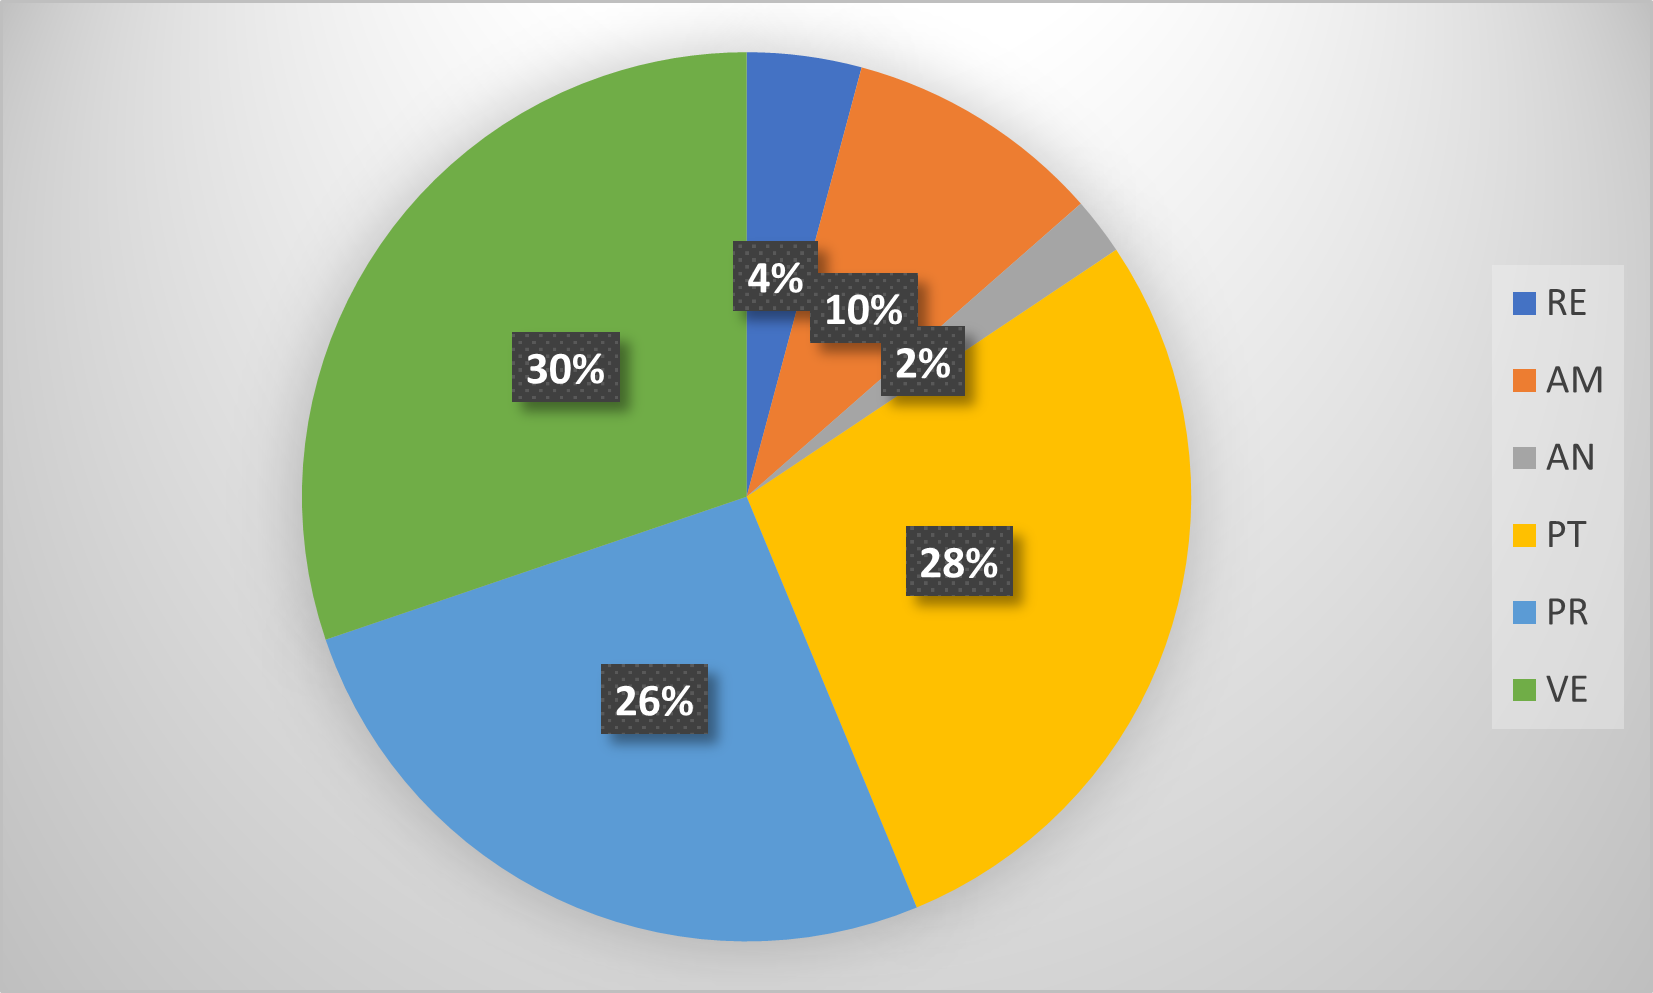
\includegraphics[width=1.0\textwidth]{Torta5.1.jpg}
    \caption{Grafico a torta della distribuzione delle ore per la quinta milestone}
\end{figure}

\newpage
\subsubsection{Preventivo economico}

\begin{table}[H]
    \renewcommand\arraystretch{1.5}
    \centering
    \begin{tabular}{|l|c|c|}
    \hline
    \rowcolor[HTML]{036400}
    \textcolor{white}{\textbf{Ruolo}} & \multicolumn{1}{l|}{\textcolor{white}{\textbf{Ore}}} & \multicolumn{1}{l|}{\textcolor{white}{\textbf{Costo (€)}}} \\ \hline
    \rowcolor[HTML]{EFEFEF}\textit{Responsabile}   & 2    & 60     \\ \hline
    \rowcolor[HTML]{C0C0C0}\textit{Amministratore} & 4.5  & 90     \\ \hline
    \rowcolor[HTML]{EFEFEF}\textit{Analista}       & 1    & 25     \\ \hline
    \rowcolor[HTML]{C0C0C0}\textit{Progettista}    & 13.5 & 337.5  \\ \hline
    \rowcolor[HTML]{EFEFEF}\textit{Programmatore}  & 12.5 & 187.5  \\ \hline
    \rowcolor[HTML]{C0C0C0}\textit{Verificatore}   & 14.5 & 217.5  \\ \hline
    \rowcolor[HTML]{EFEFEF}\textbf{Totale}         & 48   & 917.5  \\ \hline
    \end{tabular}
    \caption{Prospetto dei costi per la quinta milestone}
\end{table}

\begin{figure}[H]
    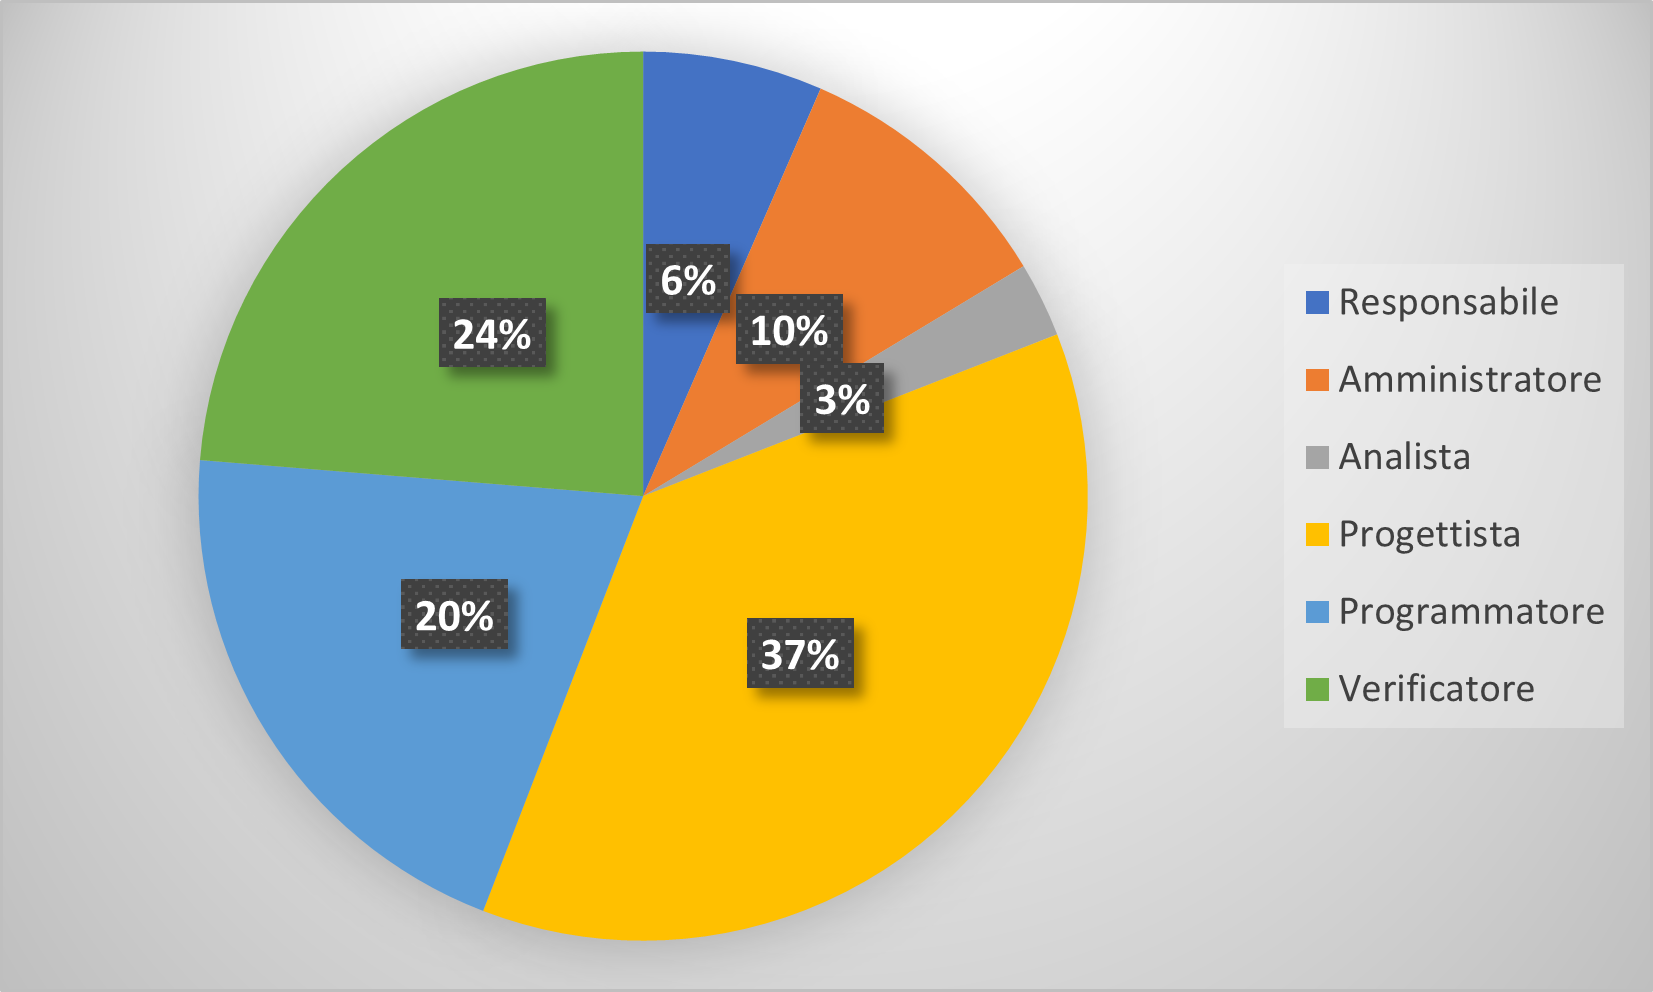
\includegraphics[width=1.0\textwidth]{Torta5.2.jpg}
    \caption{Grafico a torta della distribuzione dei costi per la quinta milestone}
\end{figure}

\subsection{Sesto periodo}

In questa fase i ruoli da ricoprire per portare a termine gli obiettivi pianificati sono:
\begin{itemize}
    \item \textit{Responsabile};
    \item \textit{Amministratore};
    \item \textit{Progettista};
    \item \textit{Programmatore};
    \item \textit{Verificatore}.
\end{itemize}

\subsubsection{Obiettivi}
Gli obiettivi di questo periodo sono:
\begin{itemize}
    \item Progettare l'architettura del prodotto;
    \item Aggiornare il documento \textit{Piano di Progetto};
    \item Aggiornare il documento \textit{Norme di Progetto};
    \item Aggiornare il documento \textit{Piano di Qualifica};
    \item Incontrare il proponente e risolvere i dubbi riscontrati nel meeting interno del 29/03/2022.
\end{itemize}

\subsubsection{Preventivo orario}

\begin{table}[H]
    \renewcommand\arraystretch{1.5}
    \centering
    \begin{tabular}{|l|c|c|c|c|c|c|c|}
    \hline
    \rowcolor[HTML]{036400}
    \textcolor{white}{\textbf{Membro}} & \multicolumn{1}{l|}{\textcolor{white}{\textbf{RE}}} & \multicolumn{1}{l|}{\textcolor{white}{\textbf{AM}}} & \multicolumn{1}{l|}{\textcolor{white}{\textbf{AN}}} & \multicolumn{1}{l|}{\textcolor{white}{\textbf{PT}}} & \multicolumn{1}{l|}{\textcolor{white}{\textbf{PR}}} & \multicolumn{1}{l|}{\textcolor{white}{\textbf{VE}}} & \multicolumn{1}{l|}{\textcolor{white}{\textbf{Totale ore persona}}} \\ \hline
    \rowcolor[HTML]{EFEFEF}\textit{Marco Mazzucato}  & - & 1   & -  & 10    & -   & 2   & 13     \\ \hline
    \rowcolor[HTML]{C0C0C0}\textit{Marco Mamprin}    & - & 1   & -  & 3     & 2   & 3   & 9     \\ \hline
    \rowcolor[HTML]{EFEFEF}\textit{Marko Vukovic}    & - & -   & -  & 12    & -   & 4   & 16     \\ \hline
    \rowcolor[HTML]{C0C0C0}\textit{Mattia Zanellato} & - & 1   & -  & 3     & 2   & 2   & 8     \\ \hline
    \rowcolor[HTML]{EFEFEF}\textit{Emanuele Pase}    & - & 2   & -  & 12    & -   & 1   & 15     \\ \hline
    \rowcolor[HTML]{C0C0C0}\textit{Riccardo Contin}  & - & -   & -  & 12    & -   & 2   & 14     \\ \hline
    \rowcolor[HTML]{EFEFEF}\textit{Lorenzo Onelia}   & 4 & -   & -  & 2     & 2   & 2   & 10    \\ \hline
    \rowcolor[HTML]{C0C0C0}\textbf{Totale ore ruolo} & 4 & 5   & 0  & 54    & 6   & 16  & 85    \\ \hline
    \end{tabular}
    \caption{Distribuzione delle ore per la sesta milestone}
\end{table}

\begin{figure}[H]
    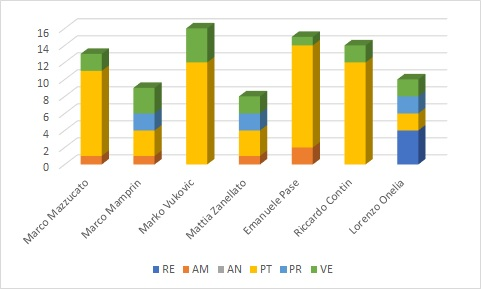
\includegraphics[width=1.0\textwidth]{Istogramma6.jpg}
    \caption{Istogramma della distribuzione delle ore per la sesta milestone}
\end{figure}

\begin{figure}[H]
    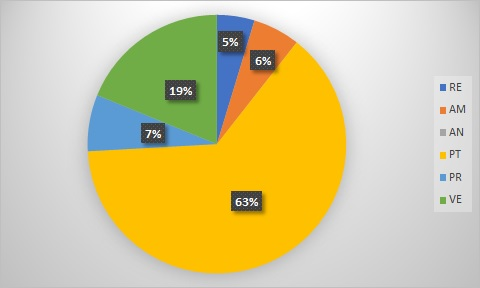
\includegraphics[width=1.0\textwidth]{Torta6.1.jpg}
    \caption{Grafico a torta della distribuzione delle ore per la sesta milestone}
\end{figure}

\newpage
\subsubsection{Preventivo economico}

\begin{table}[H]
    \renewcommand\arraystretch{1.5}
    \centering
    \begin{tabular}{|l|c|c|}
    \hline
    \rowcolor[HTML]{036400}
    \textcolor{white}{\textbf{Ruolo}} & \multicolumn{1}{l|}{\textcolor{white}{\textbf{Ore}}} & \multicolumn{1}{l|}{\textcolor{white}{\textbf{Costo (€)}}} \\ \hline
    \rowcolor[HTML]{EFEFEF}\textit{Responsabile}   & 4    & 120     \\ \hline
    \rowcolor[HTML]{C0C0C0}\textit{Amministratore} & 5  & 100     \\ \hline
    \rowcolor[HTML]{EFEFEF}\textit{Analista}       & 0    & 0     \\ \hline
    \rowcolor[HTML]{C0C0C0}\textit{Progettista}    & 54 & 1350  \\ \hline
    \rowcolor[HTML]{EFEFEF}\textit{Programmatore}  & 6 & 90  \\ \hline
    \rowcolor[HTML]{C0C0C0}\textit{Verificatore}   & 16 & 240  \\ \hline
    \rowcolor[HTML]{EFEFEF}\textbf{Totale}         & 85   & 1900  \\ \hline
    \end{tabular}
    \caption{Prospetto dei costi per la sesta milestone}
\end{table}

\begin{figure}[H]
    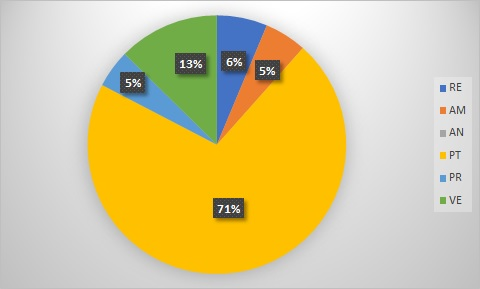
\includegraphics[width=1.0\textwidth]{Torta6.2.jpg}
    \caption{Grafico a torta della distribuzione dei costi per la sesta milestone}
\end{figure}

\subsection{Settimo periodo}

In questa fase i ruoli da ricoprire per portare a termine gli obiettivi pianificati sono:
\begin{itemize}
    \item \textit{Responsabile};
    \item \textit{Analista};
    \item \textit{Progettista};
    \item \textit{Programmatore};
    \item \textit{Verificatore}.
\end{itemize}

\subsubsection{Obiettivi}
Gli obiettivi di questo periodo sono:
\begin{itemize}
    \item Finire la progettazione dell'architettura del prodotto;
    \item Aggiornare il documento \textit{Norme di Progetto};
    \item Codificare le varie funzioni che disegnano i grafici;
    \item Trovare un adeguato algoritmo di campionamento;
    \item Incontrare il proponente per discutere dell'architettura e chiedere dei consigli sulla visualizzazione dei grafici.
\end{itemize}

\subsubsection{Preventivo orario}

\begin{table}[H]
    \renewcommand\arraystretch{1.5}
    \centering
    \begin{tabular}{|l|c|c|c|c|c|c|c|}
    \hline
    \rowcolor[HTML]{036400}
    \textcolor{white}{\textbf{Membro}} & \multicolumn{1}{l|}{\textcolor{white}{\textbf{RE}}} & \multicolumn{1}{l|}{\textcolor{white}{\textbf{AM}}} & \multicolumn{1}{l|}{\textcolor{white}{\textbf{AN}}} & \multicolumn{1}{l|}{\textcolor{white}{\textbf{PT}}} & \multicolumn{1}{l|}{\textcolor{white}{\textbf{PR}}} & \multicolumn{1}{l|}{\textcolor{white}{\textbf{VE}}} & \multicolumn{1}{l|}{\textcolor{white}{\textbf{Totale ore persona}}} \\ \hline
    \rowcolor[HTML]{EFEFEF}\textit{Marco Mazzucato}  & 6 & -   & -  & 4.5  & 4   & 3    & 17.5     \\ \hline
    \rowcolor[HTML]{C0C0C0}\textit{Marco Mamprin}    & - & -   & -  & 4    & 3   & 2    & 9     \\ \hline
    \rowcolor[HTML]{EFEFEF}\textit{Marko Vukovic}    & - & -   & -  & 4    & 6   & 2    & 12     \\ \hline
    \rowcolor[HTML]{C0C0C0}\textit{Mattia Zanellato} & - & -   & -  & 3    & 5   & 2    & 10     \\ \hline
    \rowcolor[HTML]{EFEFEF}\textit{Emanuele Pase}    & - & -   & -  & 5    & 4   & 2.5  & 11.5     \\ \hline
    \rowcolor[HTML]{C0C0C0}\textit{Riccardo Contin}  & - & -   & 1  & 3    & 5   & 2    & 11     \\ \hline
    \rowcolor[HTML]{EFEFEF}\textit{Lorenzo Onelia}   & - & -   & -  & 6    & 3   & 2    & 11    \\ \hline
    \rowcolor[HTML]{C0C0C0}\textbf{Totale ore ruolo} & 6 & 0   & 1  & 29.5 & 30  & 15.5 & 82    \\ \hline
    \end{tabular}
    \caption{Distribuzione delle ore per la settima milestone}
\end{table}

\begin{figure}[H]
    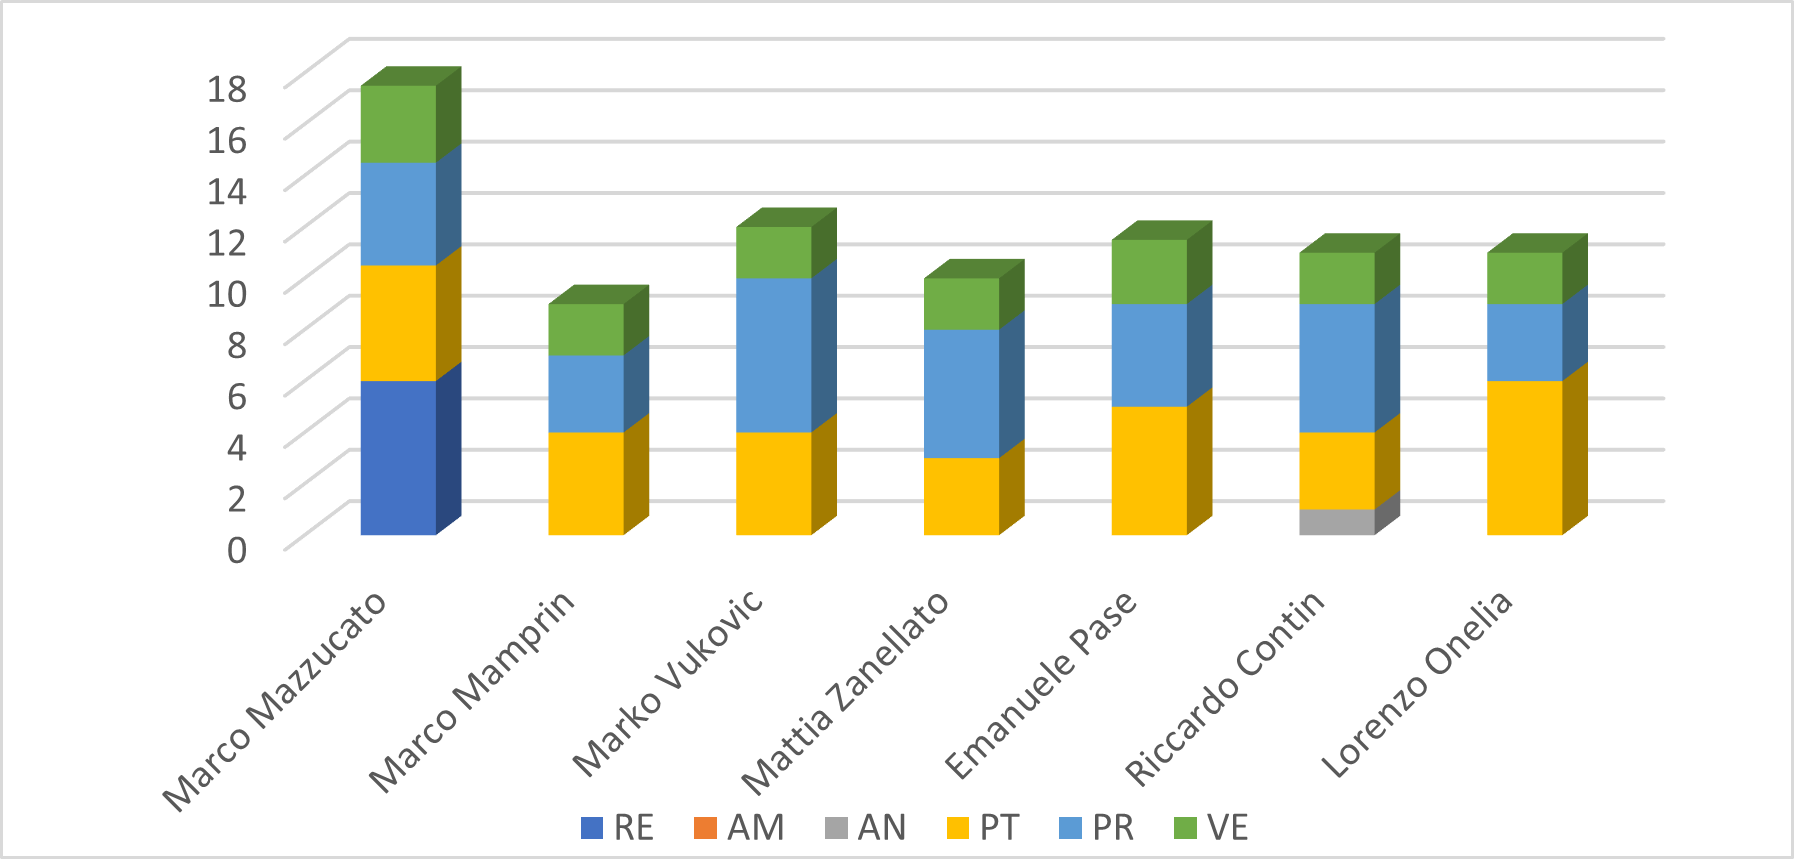
\includegraphics[width=1.0\textwidth]{Istogramma7.png}
    \caption{Istogramma della distribuzione delle ore per la settima milestone}
\end{figure}

\begin{figure}[H]
    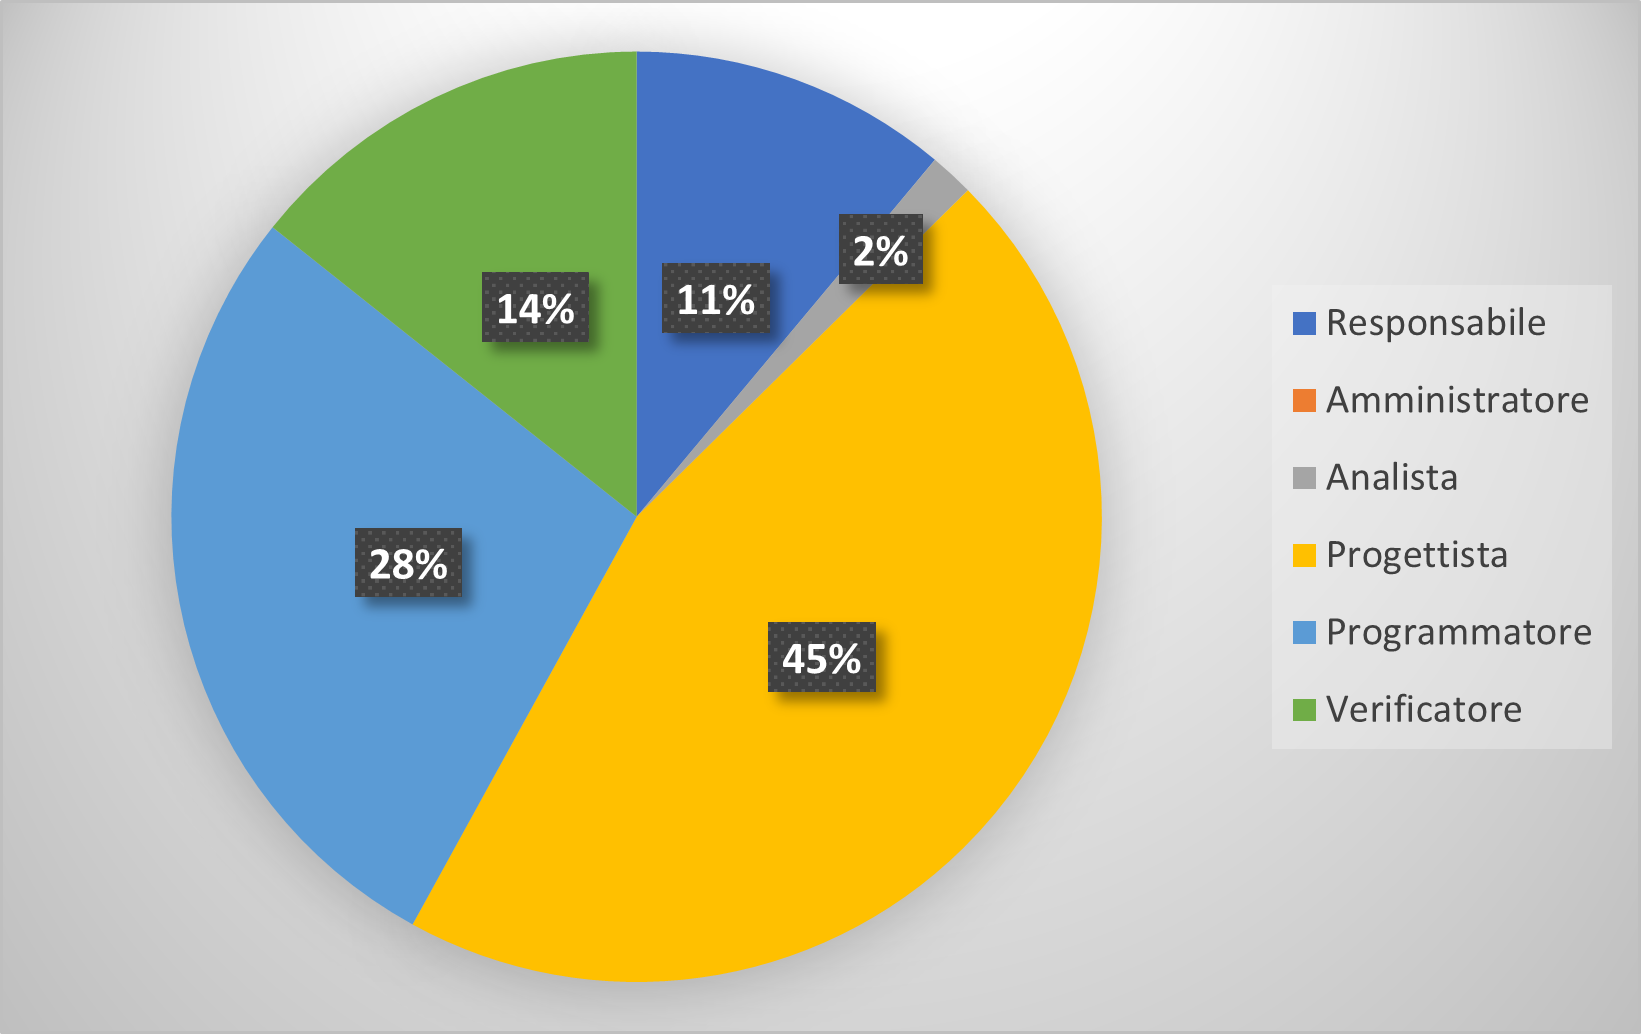
\includegraphics[width=1.0\textwidth]{Torta7.1.png}
    \caption{Grafico a torta della distribuzione delle ore per la settima milestone}
\end{figure}

\newpage
\subsubsection{Preventivo economico}

\begin{table}[H]
    \renewcommand\arraystretch{1.5}
    \centering
    \begin{tabular}{|l|c|c|}
    \hline
    \rowcolor[HTML]{036400}
    \textcolor{white}{\textbf{Ruolo}} & \multicolumn{1}{l|}{\textcolor{white}{\textbf{Ore}}} & \multicolumn{1}{l|}{\textcolor{white}{\textbf{Costo (€)}}} \\ \hline
    \rowcolor[HTML]{EFEFEF}\textit{Responsabile}   & 6    & 180     \\ \hline
    \rowcolor[HTML]{C0C0C0}\textit{Amministratore} & 0  & 0     \\ \hline
    \rowcolor[HTML]{EFEFEF}\textit{Analista}       & 1    & 25     \\ \hline
    \rowcolor[HTML]{C0C0C0}\textit{Progettista}    & 29.5 & 737.5  \\ \hline
    \rowcolor[HTML]{EFEFEF}\textit{Programmatore}  & 30 & 450  \\ \hline
    \rowcolor[HTML]{C0C0C0}\textit{Verificatore}   & 15.5 & 232.5  \\ \hline
    \rowcolor[HTML]{EFEFEF}\textbf{Totale}         & 82   & 1625  \\ \hline
    \end{tabular}
    \caption{Prospetto dei costi per la settima milestone}
\end{table}

\begin{figure}[H]
    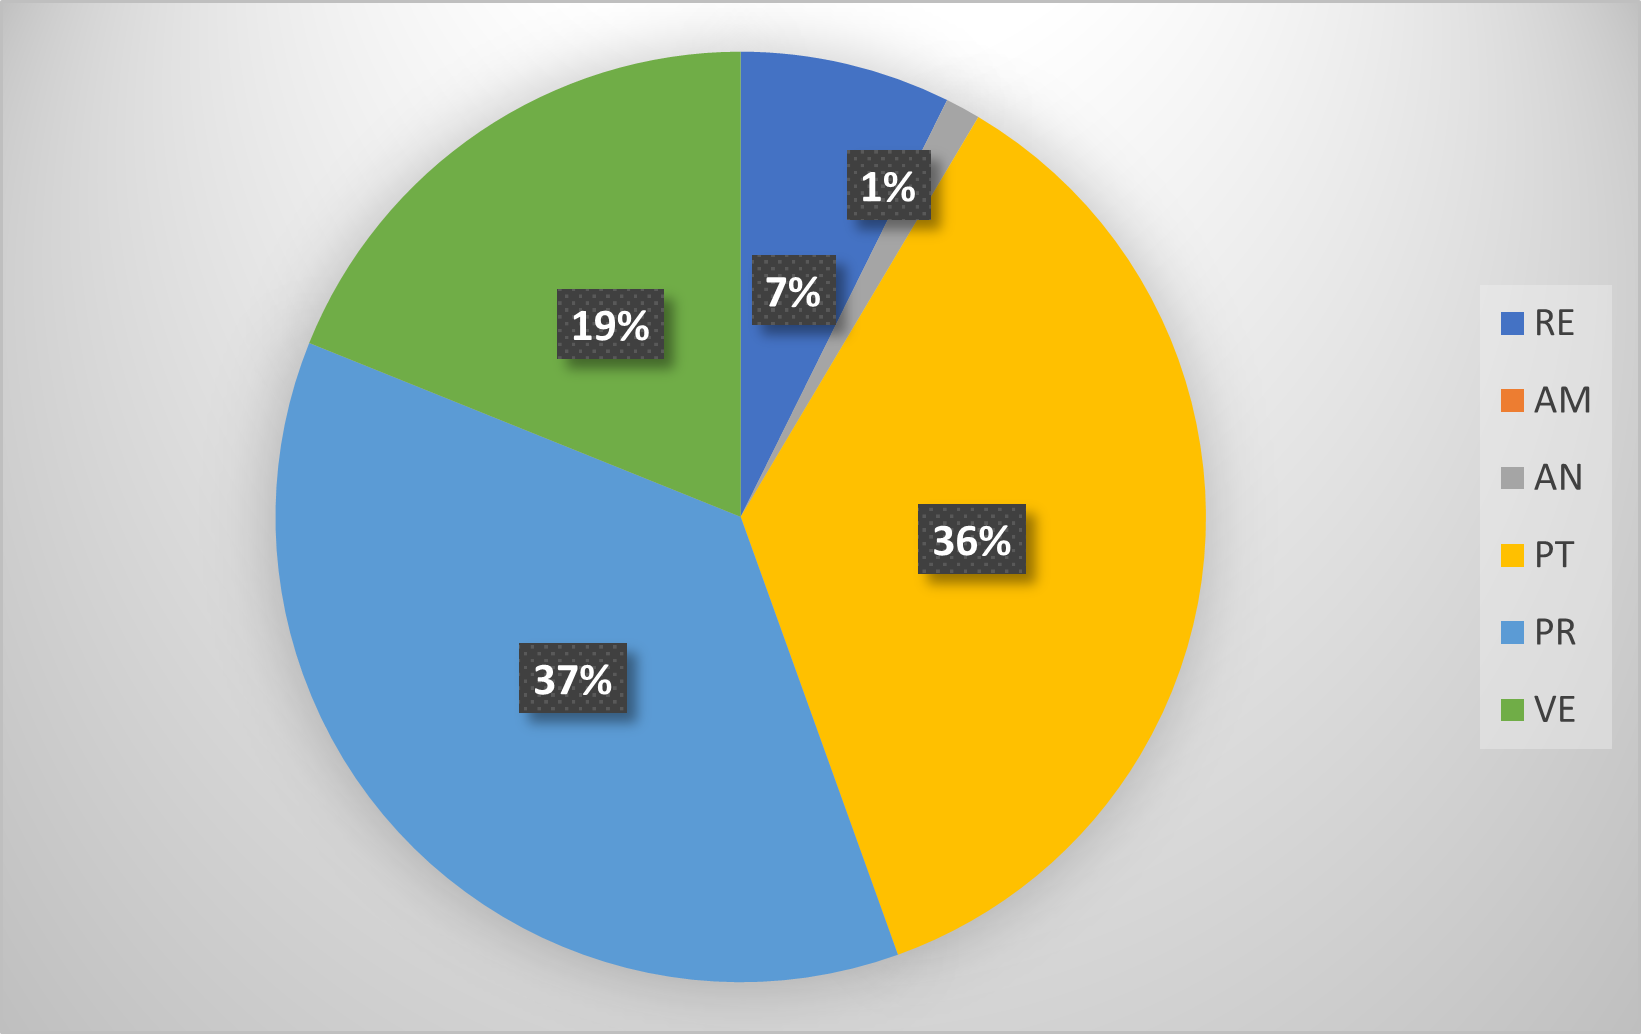
\includegraphics[width=1.0\textwidth]{Torta7.2.png}
    \caption{Grafico a torta della distribuzione dei costi per la settima milestone}
\end{figure}



\subsection{Ottavo periodo}

In questa fase i ruoli da ricoprire per portare a termine gli obiettivi pianificati sono:
\begin{itemize}
    \item \textit{Responsabile};
    \item \textit{Amministratore};
    \item \textit{Progettista};
    \item \textit{Programmatore};
    \item \textit{Verificatore}.
\end{itemize}

\subsubsection{Obiettivi}
Gli obiettivi di questo periodo sono:
\begin{itemize}
    \item Finire la progettazione modellando il diagramma di sequenza;
    \item Finire la codifica della classe "IndexedDBStorage";
    \item Codificare "Customization" e "Visualization" del diagramma delle classi;
    \item Codificare "Home Controller" e "VisualizationController" del diagramma delle classi;
    \item Codificare la parte rimanente della View;
    \item Identificare nuovi algoritmi di campionamento;
    \item Aggiornare il Cruscotto.
\end{itemize}

\subsubsection{Preventivo orario}

\begin{table}[H]
    \renewcommand\arraystretch{1.5}
    \centering
    \begin{tabular}{|l|c|c|c|c|c|c|c|}
    \hline
    \rowcolor[HTML]{036400}
    \textcolor{white}{\textbf{Membro}} & \multicolumn{1}{l|}{\textcolor{white}{\textbf{RE}}} & \multicolumn{1}{l|}{\textcolor{white}{\textbf{AM}}} & \multicolumn{1}{l|}{\textcolor{white}{\textbf{AN}}} & \multicolumn{1}{l|}{\textcolor{white}{\textbf{PT}}} & \multicolumn{1}{l|}{\textcolor{white}{\textbf{PR}}} & \multicolumn{1}{l|}{\textcolor{white}{\textbf{VE}}} & \multicolumn{1}{l|}{\textcolor{white}{\textbf{Totale ore persona}}} \\ \hline
    \rowcolor[HTML]{EFEFEF}\textit{Marco Mazzucato}  & - & 1.5 & -  & -    & 8   & 3    & 12.5     \\ \hline
    \rowcolor[HTML]{C0C0C0}\textit{Marco Mamprin}    & - & -   & -  & 4    & 5   & 3    & 12     \\ \hline
    \rowcolor[HTML]{EFEFEF}\textit{Marko Vukovic}    & - & -   & -  & -    & 10  & -    & 10     \\ \hline
    \rowcolor[HTML]{C0C0C0}\textit{Mattia Zanellato} & - & -   & -  & 3    & 6   & 2    & 11     \\ \hline
    \rowcolor[HTML]{EFEFEF}\textit{Emanuele Pase}    & 5 & -   & -  & -    & 6   & 5    & 16     \\ \hline
    \rowcolor[HTML]{C0C0C0}\textit{Riccardo Contin}  & - & -   & -  & 2    & 6   & 2    & 10     \\ \hline
    \rowcolor[HTML]{EFEFEF}\textit{Lorenzo Onelia}   & - & -   & -  & 2    & 7   & 2    & 11    \\ \hline
    \rowcolor[HTML]{C0C0C0}\textbf{Totale ore ruolo} & 5 & 1.5 & 0  & 11   & 48  & 17   & 82.5    \\ \hline
    \end{tabular}
    \caption{Distribuzione delle ore per l'ottava milestone}
\end{table}

\begin{figure}[H]
    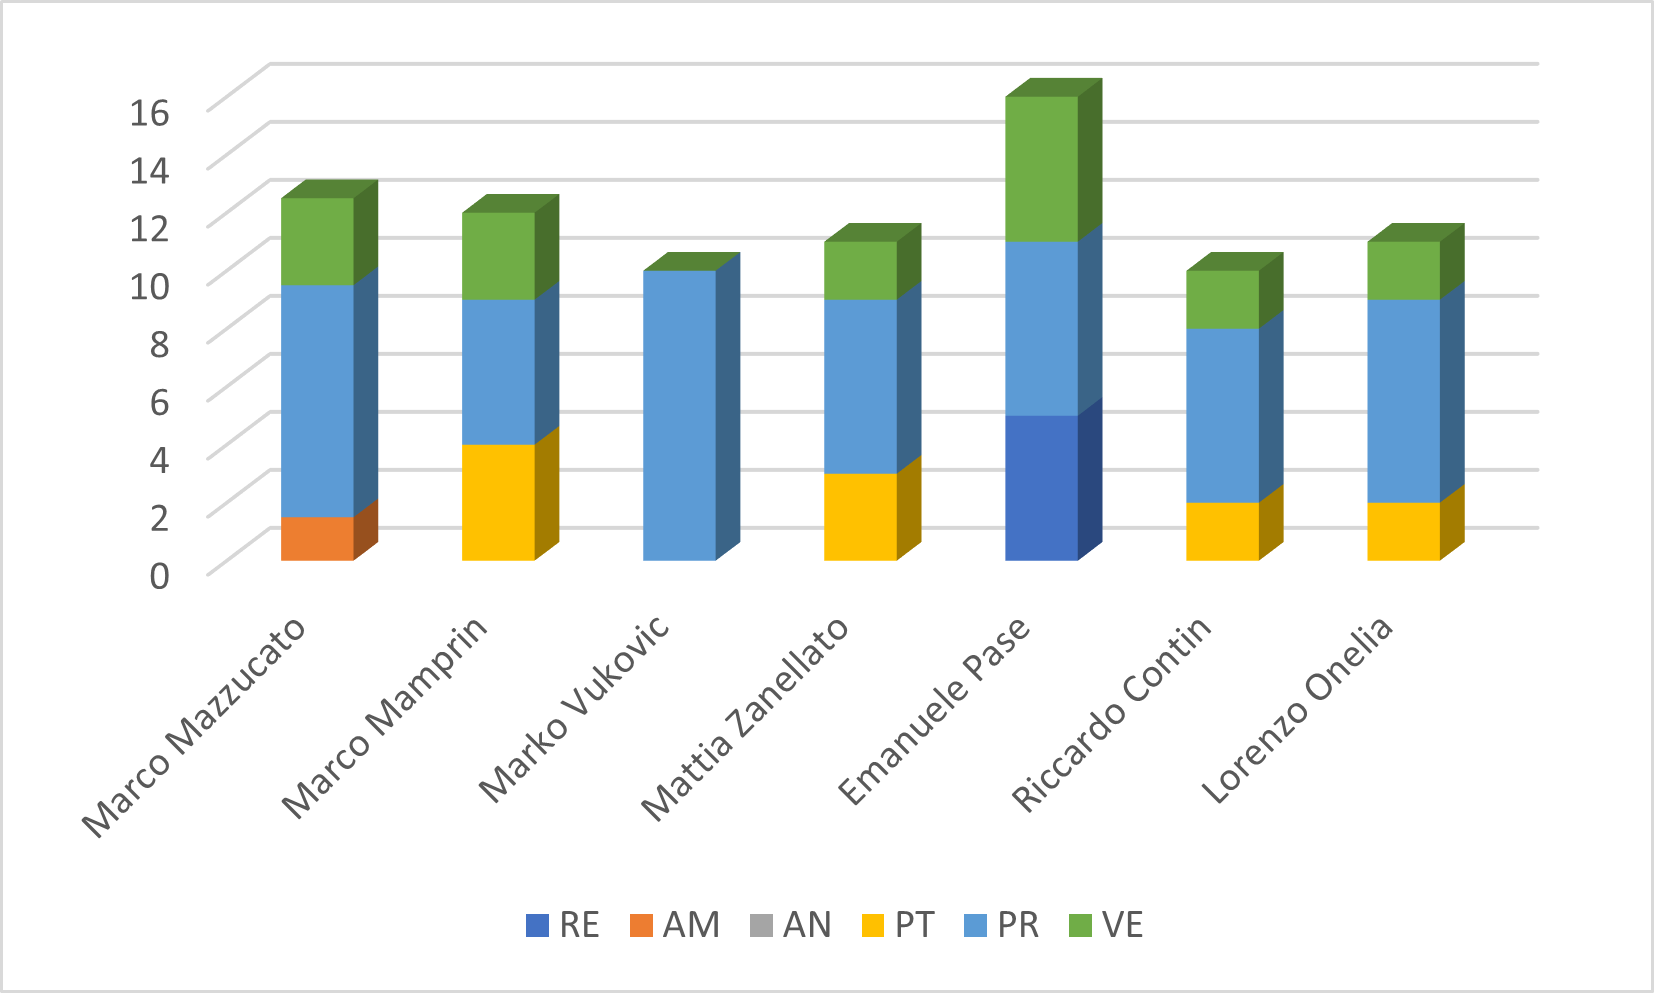
\includegraphics[width=1.0\textwidth]{Istogramma8.png}
    \caption{Istogramma della distribuzione delle ore per l'ottava milestone}
\end{figure}

\begin{figure}[H]
    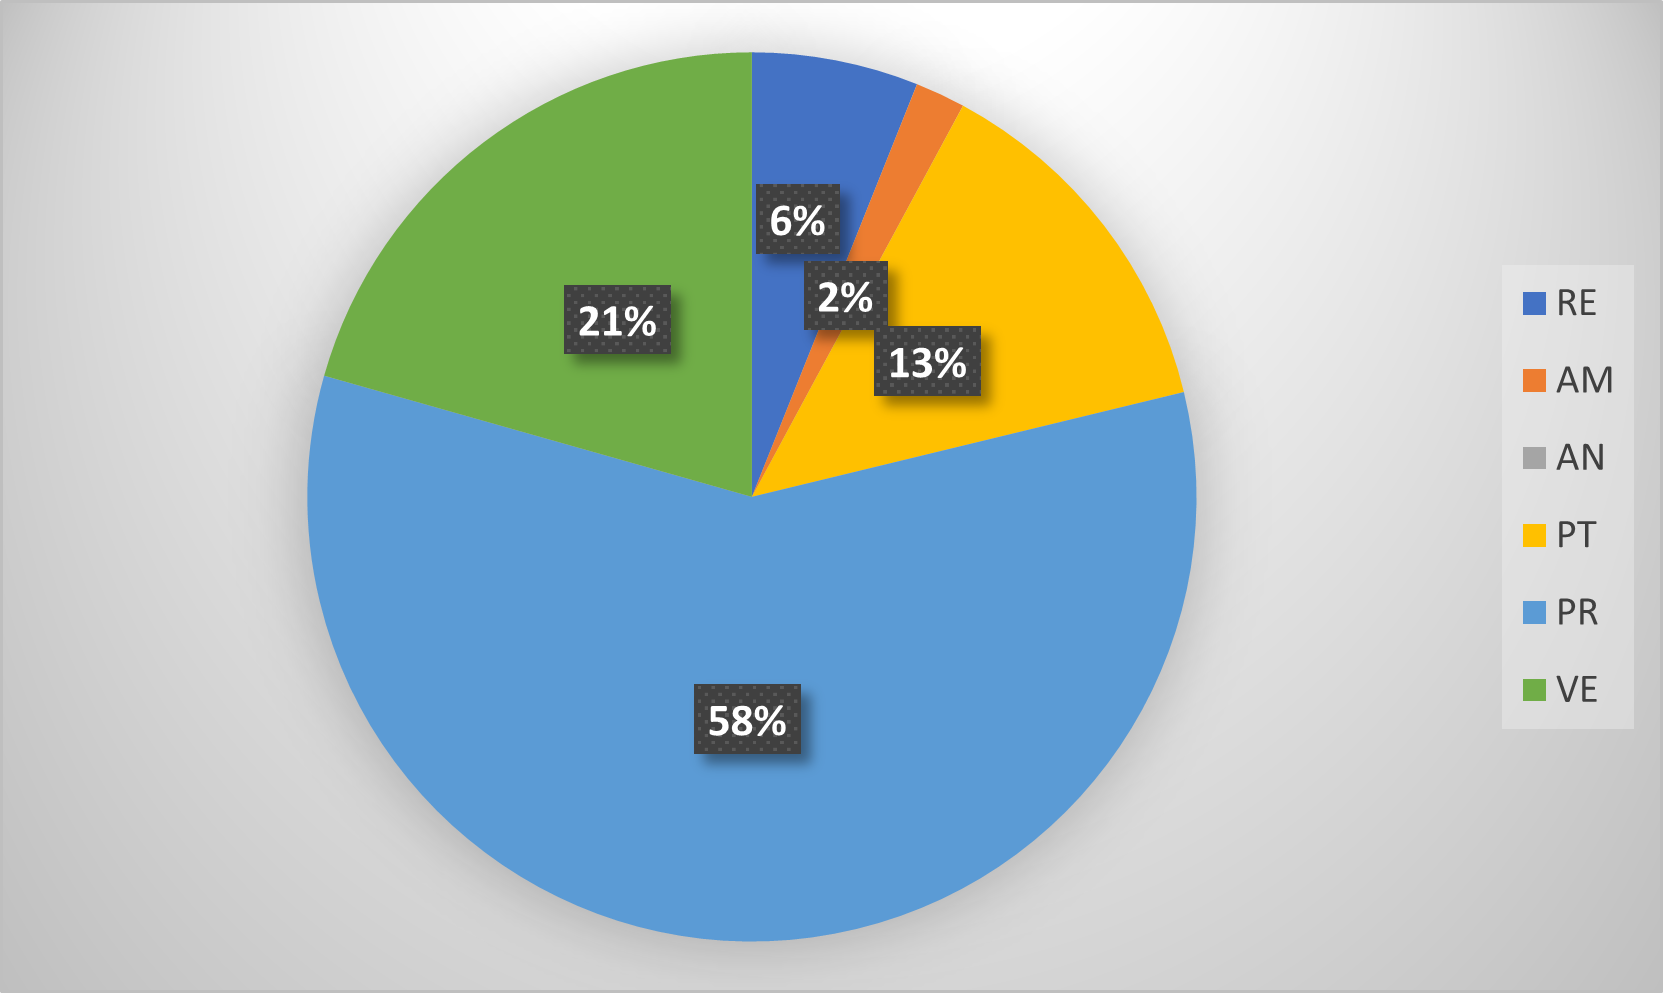
\includegraphics[width=1.0\textwidth]{Torta8.1.png}
    \caption{Grafico a torta della distribuzione delle ore per l'ottava milestone}
\end{figure}

\newpage
\subsubsection{Preventivo economico}

\begin{table}[H]
    \renewcommand\arraystretch{1.5}
    \centering
    \begin{tabular}{|l|c|c|}
    \hline
    \rowcolor[HTML]{036400}
    \textcolor{white}{\textbf{Ruolo}} & \multicolumn{1}{l|}{\textcolor{white}{\textbf{Ore}}} & \multicolumn{1}{l|}{\textcolor{white}{\textbf{Costo (€)}}} \\ \hline
    \rowcolor[HTML]{EFEFEF}\textit{Responsabile}   & 5    & 150  \\ \hline
    \rowcolor[HTML]{C0C0C0}\textit{Amministratore} & 1.5  & 30   \\ \hline
    \rowcolor[HTML]{EFEFEF}\textit{Analista}       & 0    & 0    \\ \hline
    \rowcolor[HTML]{C0C0C0}\textit{Progettista}    & 11   & 275  \\ \hline
    \rowcolor[HTML]{EFEFEF}\textit{Programmatore}  & 48   & 720  \\ \hline
    \rowcolor[HTML]{C0C0C0}\textit{Verificatore}   & 17   & 255  \\ \hline
    \rowcolor[HTML]{EFEFEF}\textbf{Totale}         & 82.5 & 1460 \\ \hline
    \end{tabular}
    \caption{Prospetto dei costi per l'ottava milestone}
\end{table}

\begin{figure}[H]
    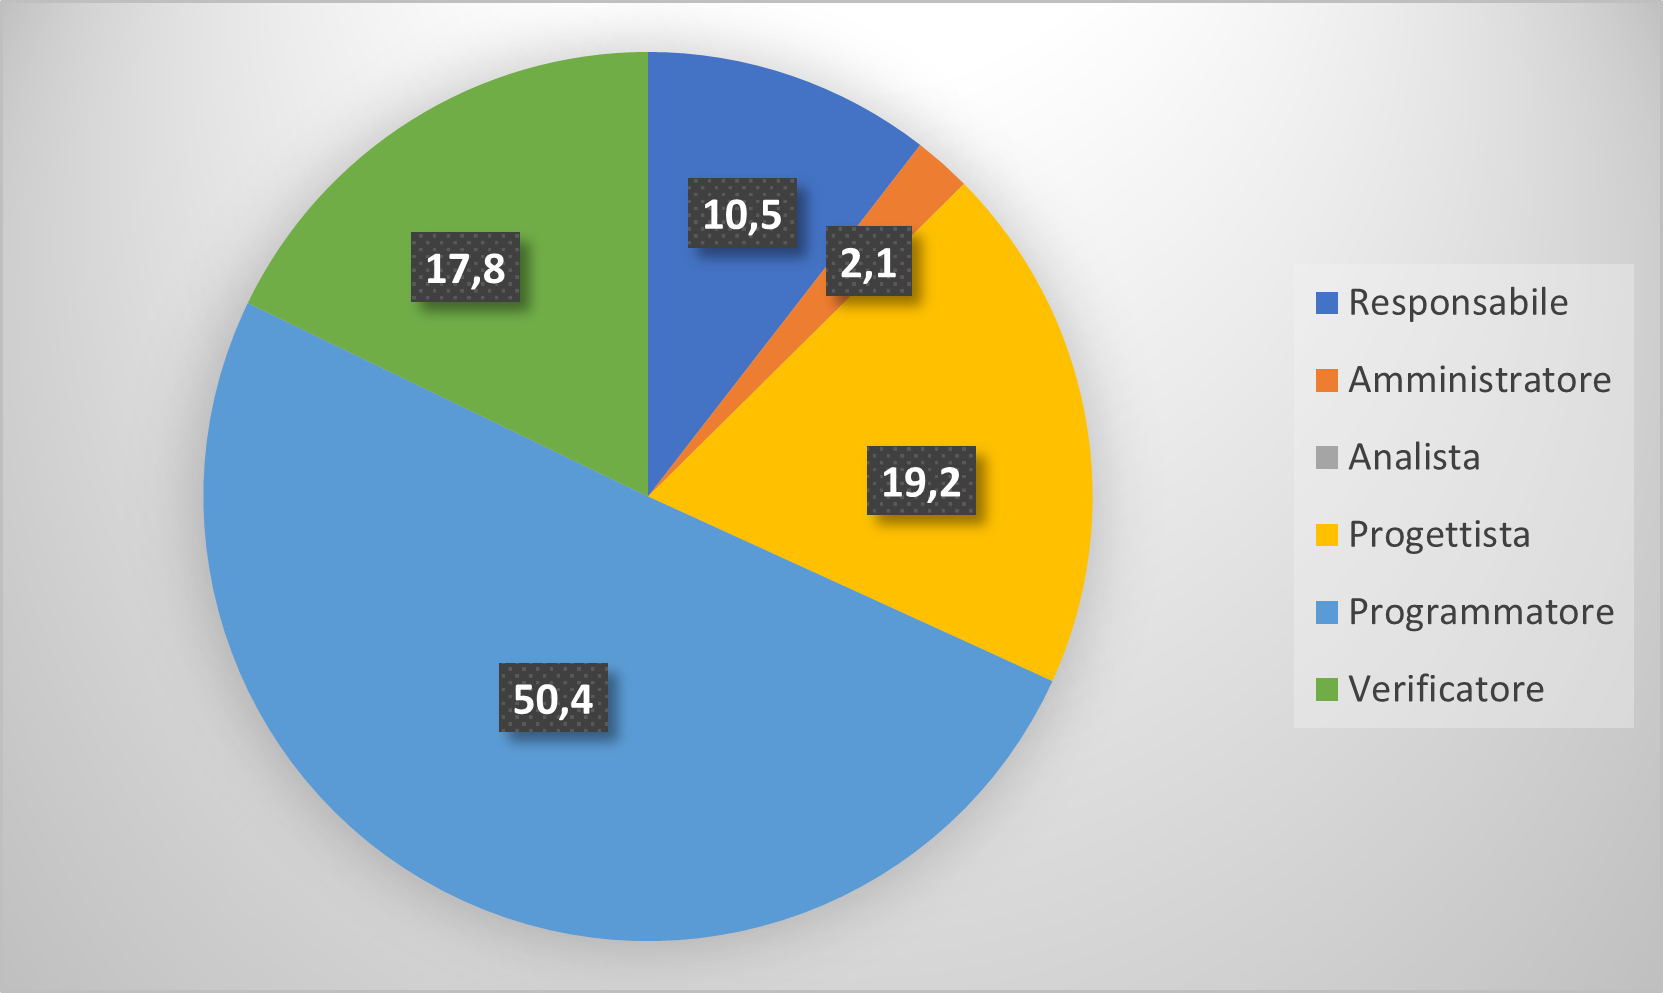
\includegraphics[width=1.0\textwidth]{Torta8.2.png}
    \caption{Grafico a torta della distribuzione dei costi per l'ottava milestone}
\end{figure}

\subsection{Nono periodo}

In questa fase i ruoli da ricoprire per portare a termine gli obiettivi pianificati sono:
\begin{itemize}
    \item \textit{Responsabile};
    \item \textit{Amministratore};
    \item \textit{Progettista};
    \item \textit{Programmatore};
    \item \textit{Verificatore}.
\end{itemize}

\subsubsection{Obiettivi}
Gli obiettivi di questo periodo sono:
\begin{itemize}
    \item Aggiornare le \textit{Norme di Progetto};
    \item Aggiornare l'\textit{Analisi dei Requisiti};
    \item Aggiornare il Cruscotto;
    \item Integrare la \textit{Specifica Architetturale};
    \item Rivedere l'architettura;
    \item Sistemare il codice già scritto;
    \item Codificare le parti mancanti;
    \item Testare il codice;
    \item Incontrare il proponente per un confronto su quanto prodotto.

\end{itemize}

\subsubsection{Preventivo orario}

\begin{table}[H]
    \renewcommand\arraystretch{1.5}
    \centering
    \begin{tabular}{|l|c|c|c|c|c|c|c|}
    \hline
    \rowcolor[HTML]{036400}
    \textcolor{white}{\textbf{Membro}} & \multicolumn{1}{l|}{\textcolor{white}{\textbf{RE}}} & \multicolumn{1}{l|}{\textcolor{white}{\textbf{AM}}} & \multicolumn{1}{l|}{\textcolor{white}{\textbf{AN}}} & \multicolumn{1}{l|}{\textcolor{white}{\textbf{PT}}} & \multicolumn{1}{l|}{\textcolor{white}{\textbf{PR}}} & \multicolumn{1}{l|}{\textcolor{white}{\textbf{VE}}} & \multicolumn{1}{l|}{\textcolor{white}{\textbf{Totale ore persona}}} \\ \hline
    \rowcolor[HTML]{EFEFEF}\textit{Marco Mazzucato}  & - & 0.5 & -  & -    & 5   & 3    & 8.5     \\ \hline
    \rowcolor[HTML]{C0C0C0}\textit{Marco Mamprin}    & - & -   & -  & 1.5  & 2   & 3.5  & 7     \\ \hline
    \rowcolor[HTML]{EFEFEF}\textit{Marko Vukovic}    & - & -   & -  & -    & -   & 5    & 5     \\ \hline
    \rowcolor[HTML]{C0C0C0}\textit{Mattia Zanellato} & - & 0.5 & -  & 1    & 3   & 3    & 7.5     \\ \hline
    \rowcolor[HTML]{EFEFEF}\textit{Emanuele Pase}    & - & -   & -  & -    & 7   & 4.5  & 11.5     \\ \hline
    \rowcolor[HTML]{C0C0C0}\textit{Riccardo Contin}  & 5 & -   & -  & 1    & 2   & 1    & 9     \\ \hline
    \rowcolor[HTML]{EFEFEF}\textit{Lorenzo Onelia}   & - & -   & -  & 1    & 7   & 2    & 10    \\ \hline
    \rowcolor[HTML]{C0C0C0}\textbf{Totale ore ruolo} & 5 & 1   & 0  & 4.5  & 26  & 22   & 58.5    \\ \hline
    \end{tabular}
    \caption{Distribuzione delle ore per la nona milestone}
\end{table}

\begin{figure}[H]
    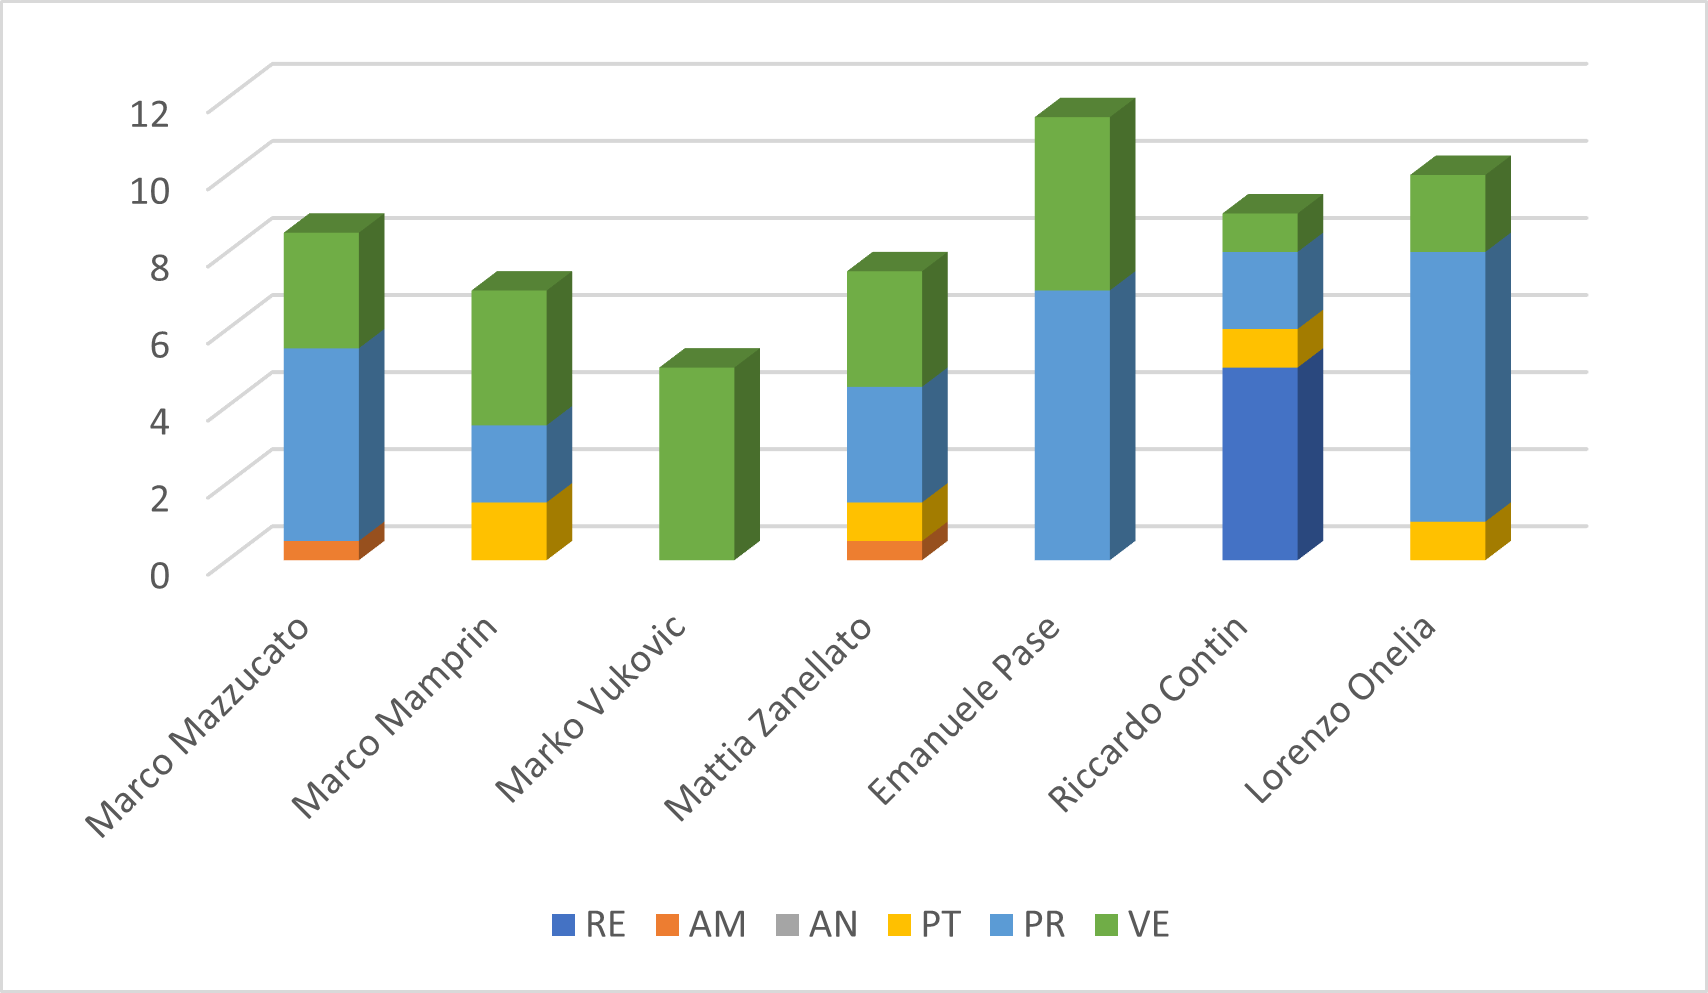
\includegraphics[width=1.0\textwidth]{Istogramma9.png}
    \caption{Istogramma della distribuzione delle ore per la nona milestone}
\end{figure}

\begin{figure}[H]
    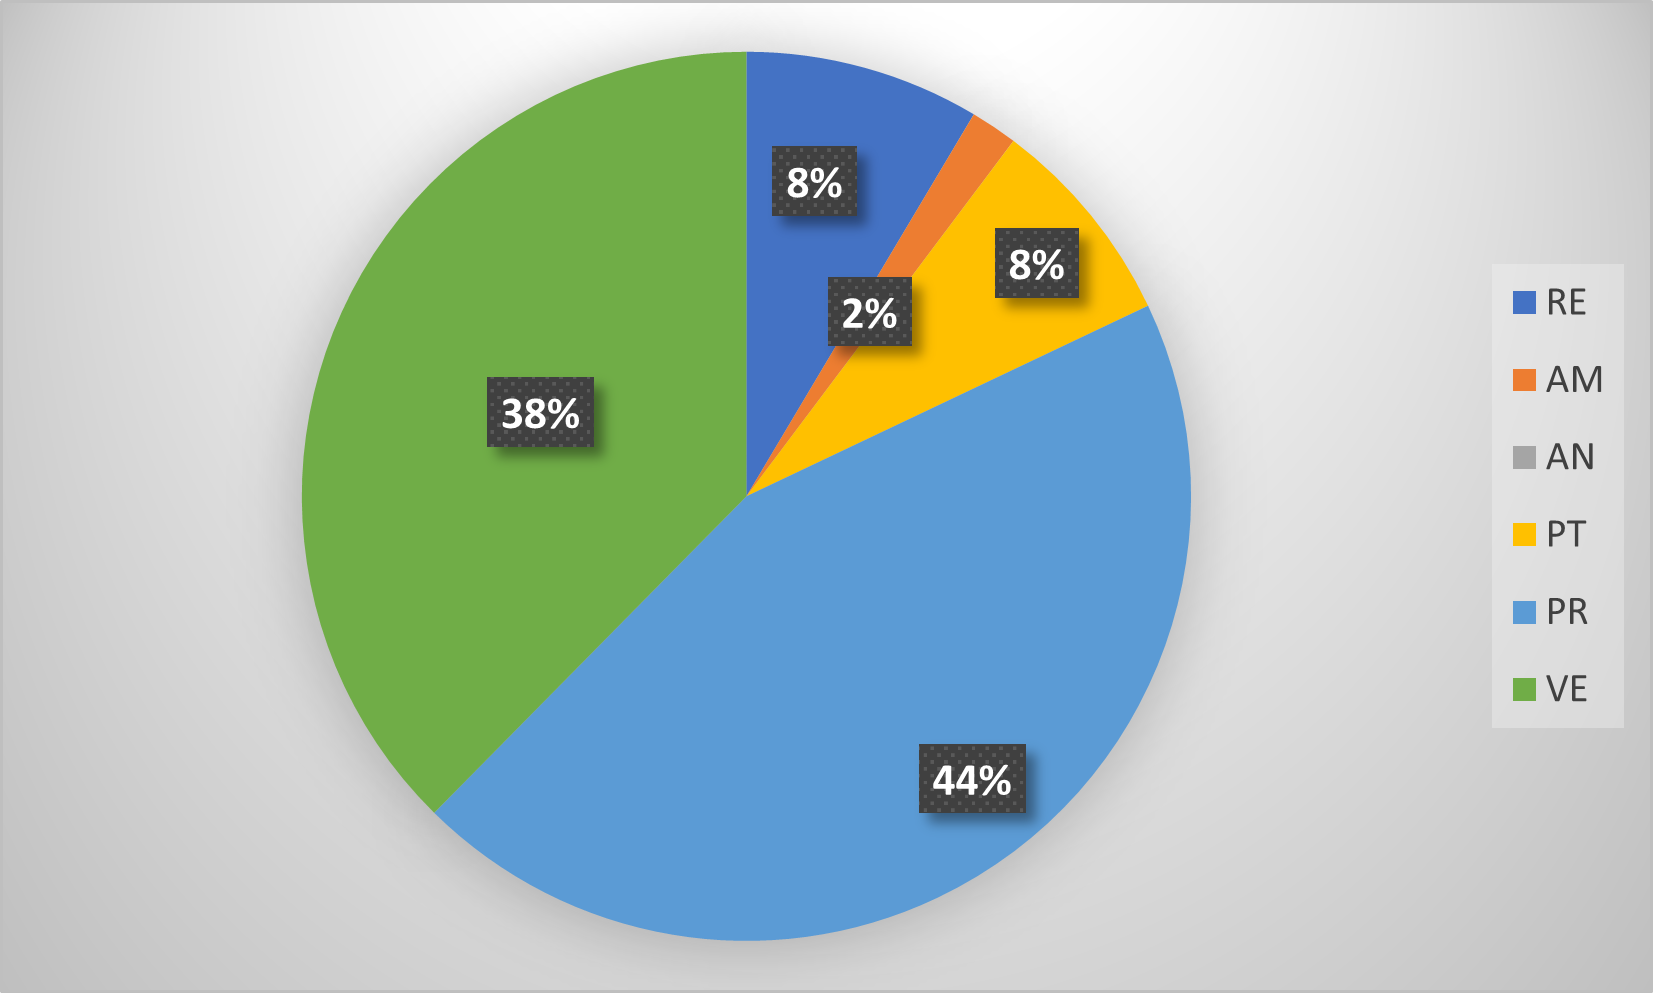
\includegraphics[width=1.0\textwidth]{Torta9.1.png}
    \caption{Grafico a torta della distribuzione delle ore per la nona milestone}
\end{figure}

\newpage
\subsubsection{Preventivo economico}

\begin{table}[H]
    \renewcommand\arraystretch{1.5}
    \centering
    \begin{tabular}{|l|c|c|}
    \hline
    \rowcolor[HTML]{036400}
    \textcolor{white}{\textbf{Ruolo}} & \multicolumn{1}{l|}{\textcolor{white}{\textbf{Ore}}} & \multicolumn{1}{l|}{\textcolor{white}{\textbf{Costo (€)}}} \\ \hline
    \rowcolor[HTML]{EFEFEF}\textit{Responsabile}   & 5    & 150    \\ \hline
    \rowcolor[HTML]{C0C0C0}\textit{Amministratore} & 1    & 20     \\ \hline
    \rowcolor[HTML]{EFEFEF}\textit{Analista}       & 0    & 0      \\ \hline
    \rowcolor[HTML]{C0C0C0}\textit{Progettista}    & 4.5  & 112.5  \\ \hline
    \rowcolor[HTML]{EFEFEF}\textit{Programmatore}  & 26   & 390    \\ \hline
    \rowcolor[HTML]{C0C0C0}\textit{Verificatore}   & 22   & 330    \\ \hline
    \rowcolor[HTML]{EFEFEF}\textbf{Totale}         & 58.5 & 1002.5 \\ \hline
    \end{tabular}
    \caption{Prospetto dei costi per la nona milestone}
\end{table}

\begin{figure}[H]
    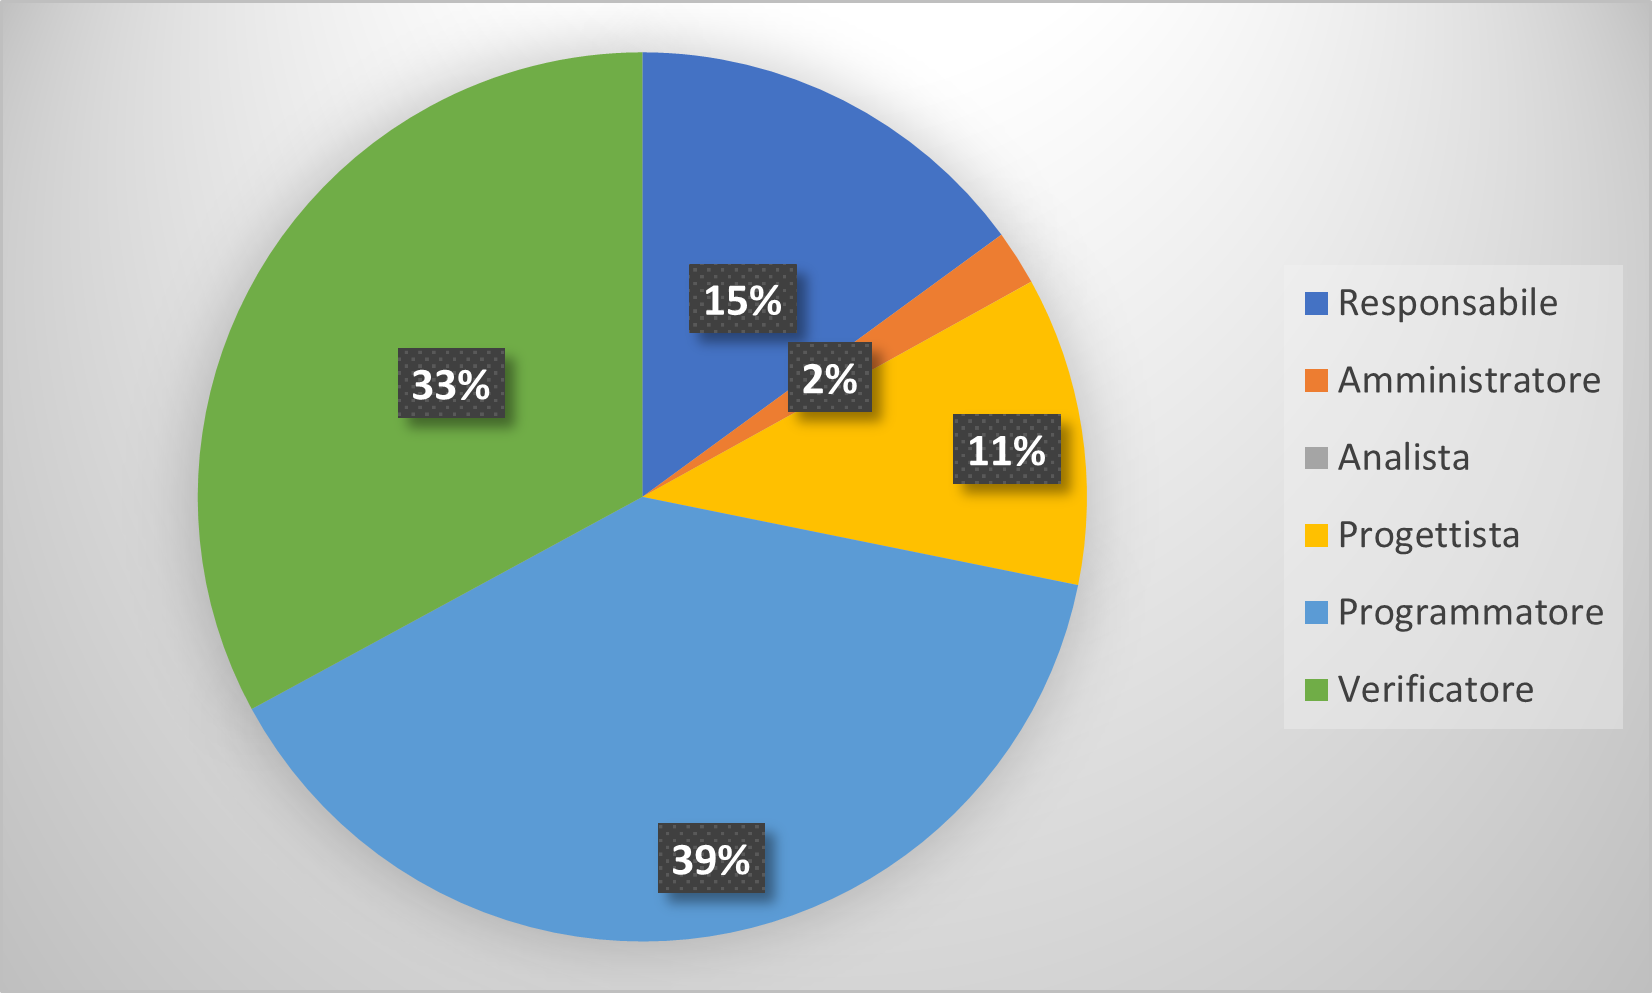
\includegraphics[width=1.0\textwidth]{Torta9.2.png}
    \caption{Grafico a torta della distribuzione dei costi per la nona milestone}
\end{figure}

\subsection{Decimo periodo}

In questa fase i ruoli da ricoprire per portare a termine gli obiettivi pianificati sono:
\begin{itemize}
    \item \textit{Responsabile};
    \item \textit{Amministratore};
    \item \textit{Progettista};
    \item \textit{Programmatore};
    \item \textit{Verificatore}.
\end{itemize}

\subsubsection{Obiettivi}
Gli obiettivi di questo periodo sono:
\begin{itemize}
    \item Terminare il documento \textit{Specifica Architetturale};
    \item Redigere la \textit{Lettera di Presentazione};
    \item Redigere il \textit{Manuale utente};
    \item Ordinare il repository  su \textbf{GitHub};
    \item Presentare la candidatura alla revisione PB.

\end{itemize}

\subsubsection{Preventivo orario}

\begin{table}[H]
    \renewcommand\arraystretch{1.5}
    \centering
    \begin{tabular}{|l|c|c|c|c|c|c|c|}
    \hline
    \rowcolor[HTML]{036400}
    \textcolor{white}{\textbf{Membro}} & \multicolumn{1}{l|}{\textcolor{white}{\textbf{RE}}} & \multicolumn{1}{l|}{\textcolor{white}{\textbf{AM}}} & \multicolumn{1}{l|}{\textcolor{white}{\textbf{AN}}} & \multicolumn{1}{l|}{\textcolor{white}{\textbf{PT}}} & \multicolumn{1}{l|}{\textcolor{white}{\textbf{PR}}} & \multicolumn{1}{l|}{\textcolor{white}{\textbf{VE}}} & \multicolumn{1}{l|}{\textcolor{white}{\textbf{Totale ore persona}}} \\ \hline
    \rowcolor[HTML]{EFEFEF}\textit{Marco Mazzucato}  & - & -   & -  & -    & 5   & 1    & 6     \\ \hline
    \rowcolor[HTML]{C0C0C0}\textit{Marco Mamprin}    & - & 0.5 & -  & 1    & -   & 2    & 3.5     \\ \hline
    \rowcolor[HTML]{EFEFEF}\textit{Marko Vukovic}    & - & -   & -  & -    & -   & -    & -     \\ \hline
    \rowcolor[HTML]{C0C0C0}\textit{Mattia Zanellato} & 4 & -   & -  & -    & -   & 2    & 6     \\ \hline
    \rowcolor[HTML]{EFEFEF}\textit{Emanuele Pase}    & - & -   & -  & -    & 2.5 & 2.5  & 5     \\ \hline
    \rowcolor[HTML]{C0C0C0}\textit{Riccardo Contin}  & - & -   & -  & -    & 1   & 2    & 3     \\ \hline
    \rowcolor[HTML]{EFEFEF}\textit{Lorenzo Onelia}   & - & -   & -  & -    & 2.5 & 2.5  & 5    \\ \hline
    \rowcolor[HTML]{C0C0C0}\textbf{Totale ore ruolo} & 4 & 0.5 & 0  & 1    & 11  & 12   & 28.5    \\ \hline
    \end{tabular}
    \caption{Distribuzione delle ore per la decima milestone}
\end{table}

\begin{figure}[H]
    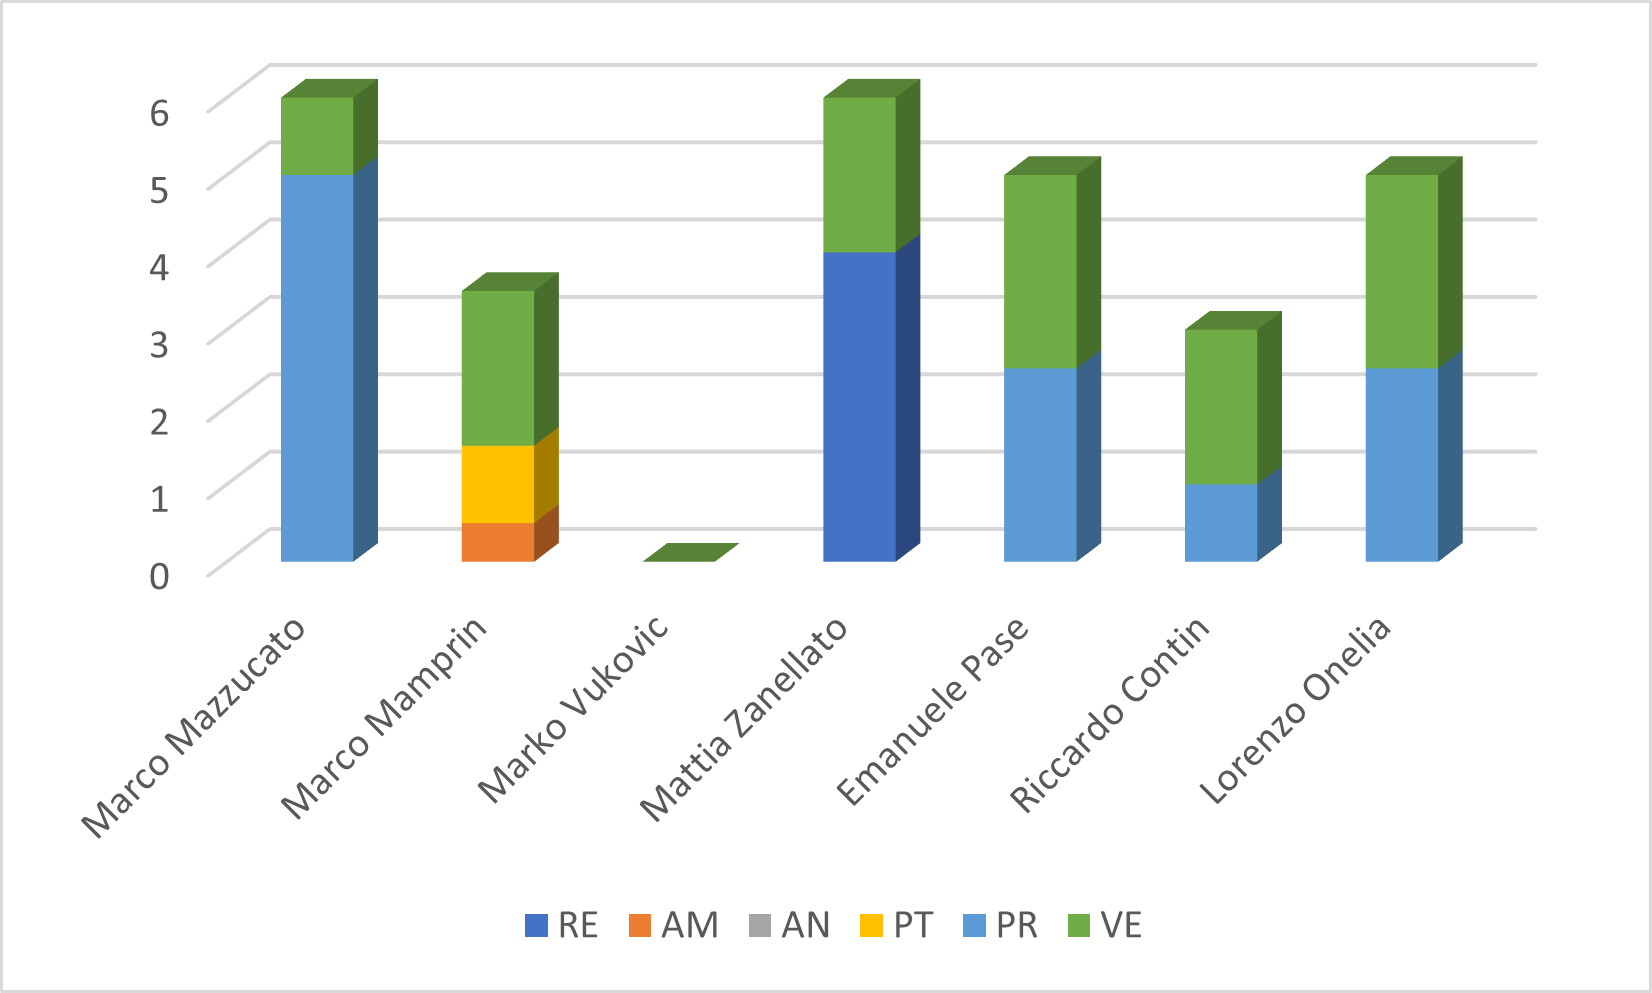
\includegraphics[width=1.0\textwidth]{Istogramma10.png}
    \caption{Istogramma della distribuzione delle ore per la decima milestone}
\end{figure}

\begin{figure}[H]
    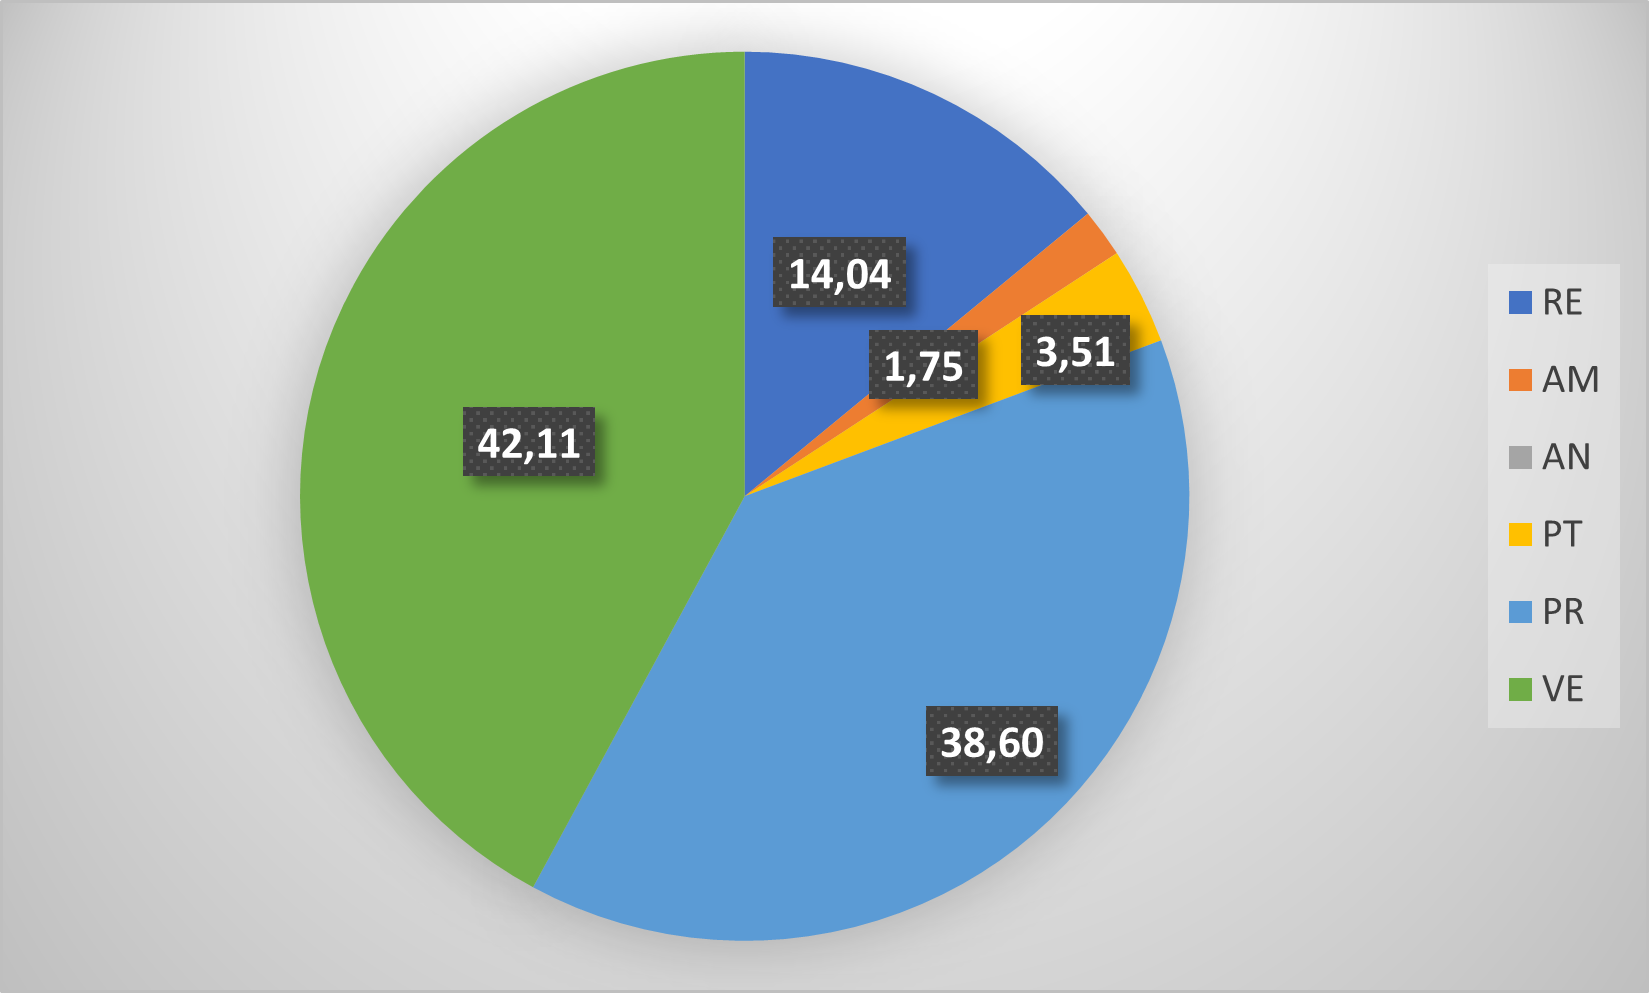
\includegraphics[width=1.0\textwidth]{Torta10.1.png}
    \caption{Grafico a torta della distribuzione delle ore per la decima milestone}
\end{figure}

\newpage
\subsubsection{Preventivo economico}

\begin{table}[H]
    \renewcommand\arraystretch{1.5}
    \centering
    \begin{tabular}{|l|c|c|}
    \hline
    \rowcolor[HTML]{036400}
    \textcolor{white}{\textbf{Ruolo}} & \multicolumn{1}{l|}{\textcolor{white}{\textbf{Ore}}} & \multicolumn{1}{l|}{\textcolor{white}{\textbf{Costo (€)}}} \\ \hline
    \rowcolor[HTML]{EFEFEF}\textit{Responsabile}   & 4    & 120    \\ \hline
    \rowcolor[HTML]{C0C0C0}\textit{Amministratore} & 0.5  & 10     \\ \hline
    \rowcolor[HTML]{EFEFEF}\textit{Analista}       & 0    & 0      \\ \hline
    \rowcolor[HTML]{C0C0C0}\textit{Progettista}    & 1    & 25     \\ \hline
    \rowcolor[HTML]{EFEFEF}\textit{Programmatore}  & 11   & 165    \\ \hline
    \rowcolor[HTML]{C0C0C0}\textit{Verificatore}   & 12   & 180    \\ \hline
    \rowcolor[HTML]{EFEFEF}\textbf{Totale}         & 28.5 & 500    \\ \hline
    \end{tabular}
    \caption{Prospetto dei costi per la decima milestone}
\end{table}

\begin{figure}[H]
    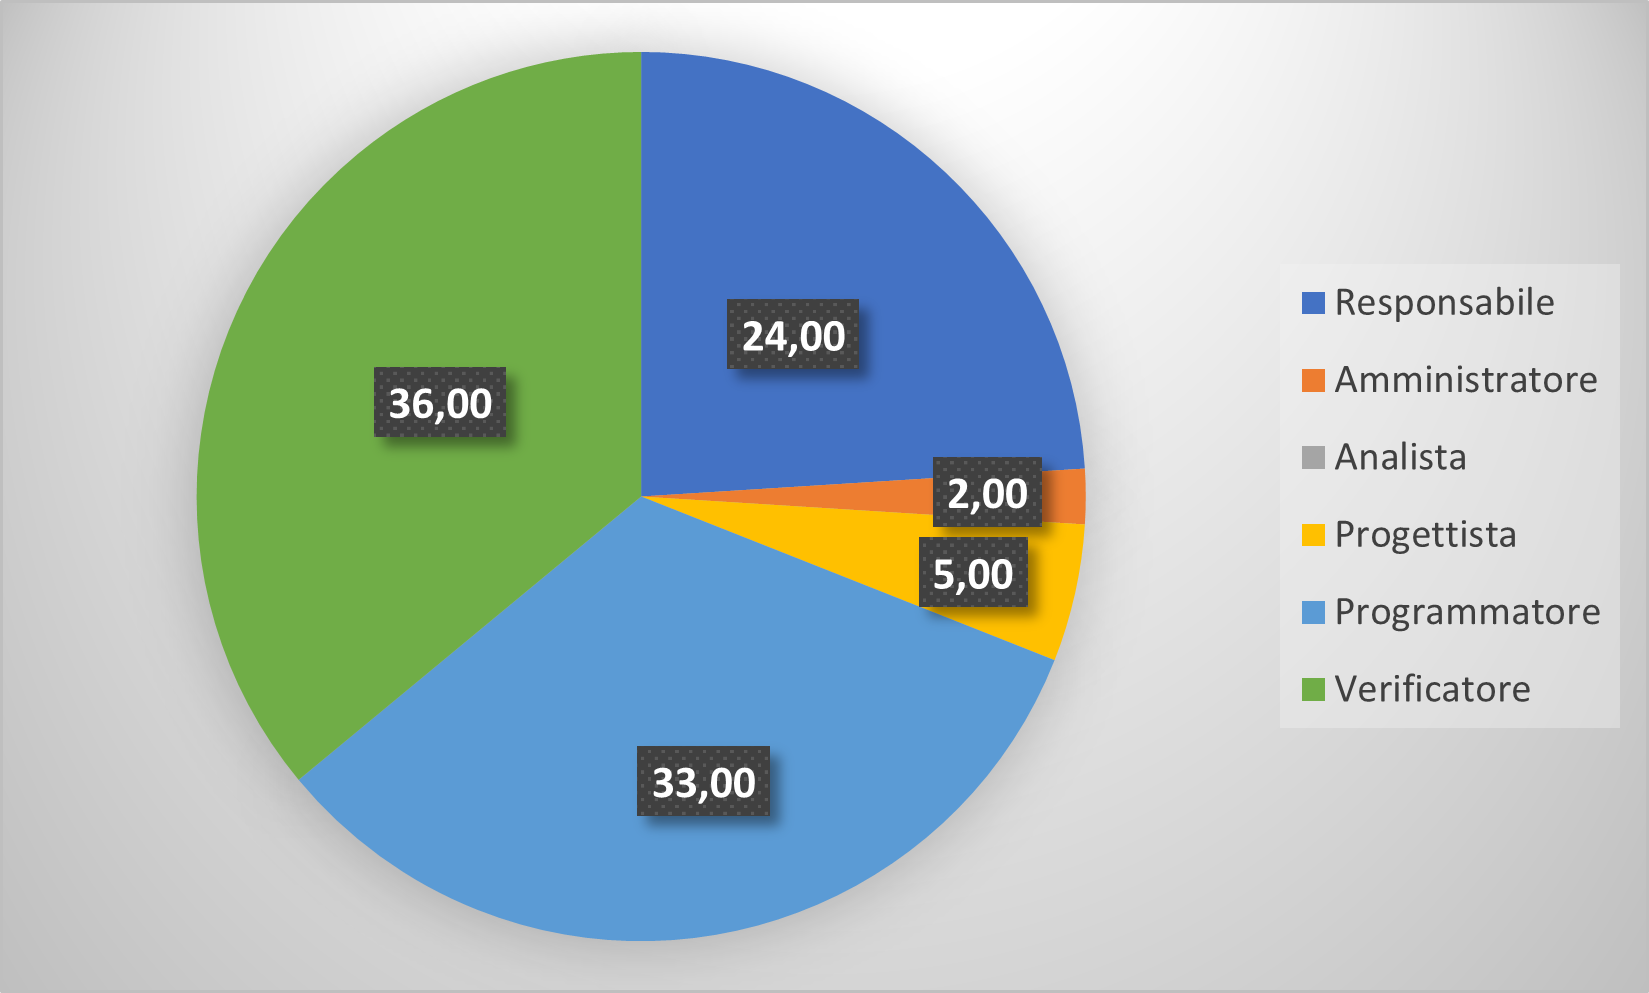
\includegraphics[width=1.0\textwidth]{Torta10.2.png}
    \caption{Grafico a torta della distribuzione dei costi per la decima milestone}
\end{figure}



\newpage
\section{Verso la CA}

\subsection{Undicesimo periodo}

In questa fase i ruoli da ricoprire per portare a termine gli obiettivi pianificati sono:
\begin{itemize}
    \item \textit{Responsabile};
    \item \textit{Progettista};
    \item \textit{Programmatore};
    \item \textit{Verificatore}.
\end{itemize}

\subsubsection{Obiettivi}
Gli obiettivi di questo periodo sono:
\begin{itemize}
    \item Redarre il \textit{Manuale Sviluppatore};
    \item Ultimare lo unit testing;
    \item Implementare il grafico Force Directed Graph;
    \item Implementare i feedback per l'utente al prodotto.

\end{itemize}

\subsubsection{Preventivo orario}

\begin{table}[H]
    \renewcommand\arraystretch{1.5}
    \centering
    \begin{tabular}{|l|c|c|c|c|c|c|c|}
    \hline
    \rowcolor[HTML]{036400}
    \textcolor{white}{\textbf{Membro}} & \multicolumn{1}{l|}{\textcolor{white}{\textbf{RE}}} & \multicolumn{1}{l|}{\textcolor{white}{\textbf{AM}}} & \multicolumn{1}{l|}{\textcolor{white}{\textbf{AN}}} & \multicolumn{1}{l|}{\textcolor{white}{\textbf{PT}}} & \multicolumn{1}{l|}{\textcolor{white}{\textbf{PR}}} & \multicolumn{1}{l|}{\textcolor{white}{\textbf{VE}}} & \multicolumn{1}{l|}{\textcolor{white}{\textbf{Totale ore persona}}} \\ \hline
    \rowcolor[HTML]{EFEFEF}\textit{Marco Mazzucato}  & -   & -   & -  & -    & 1    & 4      & 5     \\ \hline
    \rowcolor[HTML]{C0C0C0}\textit{Marco Mamprin}    & -   & -   & -  & 1    & 1    & 1      & 3     \\ \hline
    \rowcolor[HTML]{EFEFEF}\textit{Marko Vukovic}    & -   & -   & -  & -    & -    & -      & -     \\ \hline
    \rowcolor[HTML]{C0C0C0}\textit{Mattia Zanellato} & -   & -   & -  & -    & 1    & 2      & 3     \\ \hline
    \rowcolor[HTML]{EFEFEF}\textit{Emanuele Pase}    & -   & -   & -  & -    & 1.5  & 2.5    & 4     \\ \hline
    \rowcolor[HTML]{C0C0C0}\textit{Riccardo Contin}  & -   & -   & -  & -    & 3    & 4      & 7     \\ \hline
    \rowcolor[HTML]{EFEFEF}\textit{Lorenzo Onelia}   & 4.5 & -   & -  & -    & -    & 1      & 5.5    \\ \hline
    \rowcolor[HTML]{C0C0C0}\textbf{Totale ore ruolo} & 4.5 & 0   & 0  & 1    & 8.5  & 14.5   & 28.5    \\ \hline
    \end{tabular}
    \caption{Distribuzione delle ore per la undicesima milestone}
\end{table}

\begin{figure}[H]
    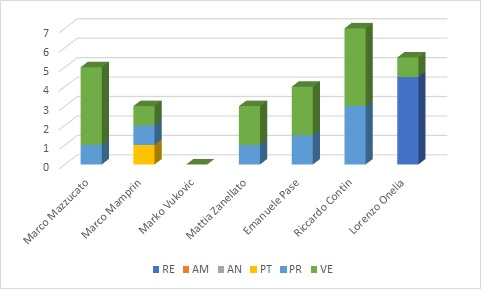
\includegraphics[width=1.0\textwidth]{Istogramma11.jpg}
    \caption{Istogramma della distribuzione delle ore per la undicesima milestone}
\end{figure}

\begin{figure}[H]
    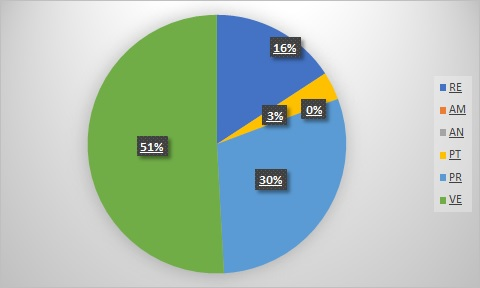
\includegraphics[width=1.0\textwidth]{Torta11.1.jpg}
    \caption{Grafico a torta della distribuzione delle ore per la undicesima milestone}
\end{figure}

\newpage
\subsubsection{Preventivo economico}

\begin{table}[H]
    \renewcommand\arraystretch{1.5}
    \centering
    \begin{tabular}{|l|c|c|}
    \hline
    \rowcolor[HTML]{036400}
    \textcolor{white}{\textbf{Ruolo}} & \multicolumn{1}{l|}{\textcolor{white}{\textbf{Ore}}} & \multicolumn{1}{l|}{\textcolor{white}{\textbf{Costo (€)}}} \\ \hline
    \rowcolor[HTML]{EFEFEF}\textit{Responsabile}   & 4.5    & 135    \\ \hline
    \rowcolor[HTML]{C0C0C0}\textit{Amministratore} & 0  & 0     \\ \hline
    \rowcolor[HTML]{EFEFEF}\textit{Analista}       & 0    & 0      \\ \hline
    \rowcolor[HTML]{C0C0C0}\textit{Progettista}    & 1    & 25     \\ \hline
    \rowcolor[HTML]{EFEFEF}\textit{Programmatore}  & 7.5   & 112.5    \\ \hline
    \rowcolor[HTML]{C0C0C0}\textit{Verificatore}   & 14.5   & 217.5    \\ \hline
    \rowcolor[HTML]{EFEFEF}\textbf{Totale}         & 27.5 & 490   \\ \hline
    \end{tabular}
    \caption{Prospetto dei costi per la undicesima milestone}
\end{table}

\begin{figure}[H]
    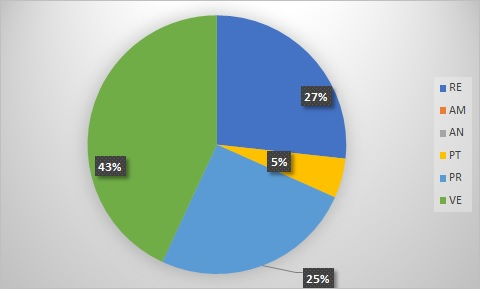
\includegraphics[width=1.0\textwidth]{Torta11.2.jpg}
    \caption{Grafico a torta della distribuzione dei costi per la undicesima milestone}
\end{figure}
